\documentclass{patmorin}
\usepackage[T1]{fontenc}
\usepackage[utf8]{inputenc}
\usepackage{amsmath,wrapfig}
\usepackage{amsfonts}
\usepackage{amsthm}
\usepackage{graphicx}
\usepackage{enumerate}
\usepackage{amsfonts}
\usepackage{amsthm,mathtools}
\usepackage{pat}
\usepackage{paralist}
\usepackage{stmaryrd}
\usepackage{thm-restate}

\usepackage[longnamesfirst,numbers,sort&compress]{natbib}
\usepackage[noabbrev,capitalise]{cleveref}

\usepackage{doi} % To make plainnat handle doi's properly 

\usepackage[mathlines]{lineno}
% \setlength{\linenumbersep}{2em}
\linenumbers
% \rightlinenumbers
% \linenumbers
\newcommand*\patchAmsMathEnvironmentForLineno[1]{%
 \expandafter\let\csname old#1\expandafter\endcsname\csname #1\endcsname
 \expandafter\let\csname oldend#1\expandafter\endcsname\csname end#1\endcsname
 \renewenvironment{#1}%
    {\linenomath\csname old#1\endcsname}%
    {\csname oldend#1\endcsname\endlinenomath}}% 
\newcommand*\patchBothAmsMathEnvironmentsForLineno[1]{%
 \patchAmsMathEnvironmentForLineno{#1}%
 \patchAmsMathEnvironmentForLineno{#1*}}%
\AtBeginDocument{%
\patchBothAmsMathEnvironmentsForLineno{equation}%
\patchBothAmsMathEnvironmentsForLineno{align}%
\patchBothAmsMathEnvironmentsForLineno{flalign}%
\patchBothAmsMathEnvironmentsForLineno{alignat}%
\patchBothAmsMathEnvironmentsForLineno{gather}%
\patchBothAmsMathEnvironmentsForLineno{multline}%
}


\allowdisplaybreaks
%\sloppy
%%%%%%%%%%
\makeatletter
\def\NAT@spacechar{~}
\makeatother
%%%%%%%%%%
\crefname{lem}{Lemma}{Lemmas}
\crefname{thm}{Theorem}{Theorems}
\crefname{cor}{Corollary}{Corollaries}
\crefname{conj}{Conjecture}{Conjectures}
\crefname{obs}{Observation}{Observations}
\crefname{prop}{Proposition}{Propositions}
\crefname{clm}{Claim}{Claims}
\crefname{openproblem}{Open Problem}{Open Problems}
\crefformat{equation}{(#2#1#3)}
\Crefformat{equation}{Equation #2(#1)#3}

\setlength{\parskip}{0.82ex}

 \newcommand{\note}[2]{{\color{red}[#1:~#2]}}
% \newcommand{\notex}[2]{{\color{blue}[#1:~#2]}}
\newcommand{\notex}[2]{}

\DeclareMathOperator{\dist}{dist}
\DeclareMathOperator{\depth}{depth}
\DeclareMathOperator{\ff}{f}
\DeclareMathOperator{\tw}{tw}
\DeclareMathOperator{\pw}{pw}
\DeclareMathOperator{\qn}{qn}
\DeclarePairedDelimiter{\ceil}{\lceil}{\rceil}
\DeclarePairedDelimiter{\floor}{\lfloor}{\rfloor}

\newcommand{\PRlabel}[1]{\label{PR:#1}}
\newcommand{\PRref}[1]{(PR\ref{PR:#1})}

\newcommand{\jlabel}[1]{\label{j:#1}}
\newcommand{\jref}[1]{(J\ref{j:#1})}

\newcommand{\tlabel}[1]{\label{t:#1}}
\newcommand{\tref}[1]{(T\ref{t:#1})}
\newcommand{\ylabel}[1]{\label{y:#1}}
\newcommand{\yref}[1]{(Y\ref{y:#1})}

\newcommand{\PP}{\mathcal{P}}

\renewcommand{\ge}{\geqslant}
\renewcommand{\le}{\leqslant}
\renewcommand{\geq}{\geqslant}
\renewcommand{\leq}{\leqslant}


% \newcommand*{\doi}[1]{\href{https://dx.doi.org/#1}{\verb+doi: #1+}}


%\newcommand{\Bagsize}{\ensuremath{\frac{k^3}{6} + \frac{3k^2}{2} + \frac{13k}{3} + 4}}
% \newcommand{\bagsize}{\ensuremath{k^3/6 + 3k^2/2 + 13k/3 + 4}}
\newcommand{\treewidth}{\ensuremath{\binom{k+4}{3}}-1}

\title{\MakeUppercase{The Structure of $k$-Planar Graphs}}

\author{Vida Dujmovi\'c%
        \thanks{School of Computer Science and Electrical Engineering,
                University of Ottawa, Ottawa, Canada (\texttt{vida.dujmovic@uottawa.ca}).
                Research  supported by NSERC and the Ontario Ministry of Research and Innovation.},\,\,
        Pat Morin%
        \thanks{School of Computer Science, Carleton University, Ottawa, Canada (\texttt{morin@scs.carleton.ca}).                 Research  supported by NSERC and the Ontario Ministry of Research and Innovation.},\,\, and
        David R. Wood\thanks{School of Mathematics, Monash University, Melbourne, Australia (\texttt{david.wood@monash.edu}). Research supported by the Australian Research Council.}
}

\begin{document}
\begin{titlepage}
\maketitle

\begin{abstract}
Dujmovi\'c~et~al.~(FOCS 2019) recently proved that every planar graph is a subgraph of the strong product of a graph of bounded treewidth and a path. This tool has been used to solve longstanding problems on queue layouts, non-repetitive colouring, $p$-centered colouring, and implicit graph encoding. We extend this result for $k$-planar graphs, where a graph is \emph{$k$-planar} if it has a drawing in the plane in which each edge is involved in at most $k$ crossings. In particular, we prove that every $k$-planar graph is a subgraph of the strong product of a graph of treewidth $O(k^5)$ and a path. This is the first result of this type for a non-minor-closed class of graphs. It implies, amongst other results, that $k$-planar graphs have non-repetitive chromatic number upper-bounded by a function of $k$. All these results generalise for drawings of graphs on arbitrary surfaces. In fact, we work in a much more general setting based on so-called shortcut systems that are of independent interest. 
\end{abstract}
\end{titlepage}

% \tableofcontents
% \newpage

%\setcounter{\page}{1}
\section{Introduction}
\label{Introduction}

A graph is \emph{$k$-planar} if it has a drawing in the plane in which each edge is involved in at most $k$ crossings. Such graphs provide a natural generalisation of planar graphs, and are important in graph drawing research; see the recent bibliography on 1-planar graphs and the 140 references therein \citep{kobourov.liotta.ea:annotated}. The present paper studies the structure of $k$-planar graphs and other more general classes of graphs. 
\notex{PM}{I removed the following sentences because neither Vida nor could find anything about $k$-planar graphs in \cite{FP08} and, in any case, the proof is easy.  This could easily upset a referee.
% \note{PM}{I must be missing something.  The planarized graph $G'$ has $O(kn)$ vertices.  Let $S$ be the set of non-dummy vertices and take a separation $(A,B)$ of $G'$ with $|A\cap B|=O(\sqrt{kn})$, $|S\cap (A\setminus B)|\le 2|S|/3$ and $|S\cap (B\setminus A)|\le 2|S|/3$.  Now take $X=A\cap B$ plus the endpoints of every edge of $G$ that contains a dummy vertex in $A\cap B$.  $|X|\le 5|A\cap B|=O(\sqrt{kn})$ and $X$ is a separator of $G$.} \note{DW}{I think you have just found a new proof of this fact. Note that you are actually using that $G'$ has treewidth $O(\sqrt{kn})$ and then applying the Robertson-Seymour separator lemma for graphs of given treewidth (so that $|S\cap (A\setminus B)|\le 2|S|/3$ and $|S\cap (B\setminus A)|\le 2|S|/3$). }
Various structural results about planar graphs generalise for $k$-planar graphs. For example, \citet{FP08} generalised the Lipton-Tarjan separator theorem to show that every $k$-planar graph with $n$ vertices has a balanced separator of order $O(\sqrt{kn})$.}

Our main results extends the following recent theorem of \citet{dujmovic.joret.ea:planar} to a setting that includes $k$-planar graphs.
 % as well as some other interesting non-minor-closed graph families.

\begin{thm}[\citep{dujmovic.joret.ea:planar}] 
\label{PlanarBasic}
Every planar graph is a subgraph of $H\boxtimes P$, for some graph $H$ of treewidth at most $8$ and for some path $P$. 
\end{thm}

Here $\boxtimes$ is the strong product, and treewidth is an invariant that measures how `tree-like' a given graph is; see \cref{Tools} for formal definitions and see \cref{ProductExample} for an example. Loosely speaking, \cref{PlanarBasic} says that every planar graph is contained in the product of a tree-like graph and a path. This enables combinatorial results for graphs of bounded 
treewidth to be generalised for planar graphs (with different constants). \cref{PlanarBasic} has been the key tool in solving several well-known open problems. In particular, \citet{dujmovic.joret.ea:planar} use it to prove that planar graphs have bounded queue-number (resolving a conjecture of \citet{HLR92} from 1992);  \citet{dujmovic.esperet.ea:planar} use it to prove that planar graphs have bounded non-repetitive chromatic number (resolving a conjecture of \citet{AGHR-RSA02} from 2002); and \citet{bonamy.gavoille.ea:shorter} use it to find shorter implicit representations of planar graphs (making progress on a sequence of results going back to 1988 \citep{kannan.naor.ea:implicit-stoc,kannan.naor.ea:implicit}). 

% \begin{wrapfigure}{r}{0.5\textwidth} 
\begin{figure}[hbtp]
\begin{center}
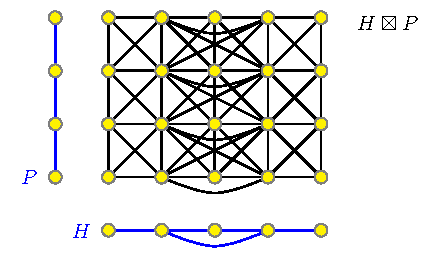
\includegraphics{ProductExample}
\end{center}
\caption{Example of a strong product.}
\label{ProductExample}
\end{figure}
% \end{wrapfigure}

We extend \cref{PlanarBasic} as follows. 

\begin{thm}
\label{kPlanarBasic}
Every $k$-planar graph is a subgraph of $H\boxtimes P$, for some graph $H$ of treewidth $(18k^2+30k)\binom{k+4}{3}-1$ and for some path $P$. 
\end{thm}

Although $k$-planar graphs are the most high-profile target for a generalization of \cref{PlanarBasic}, we actually prove a substantially stronger result than \cref{kPlanarBasic} using the following definition. A non-empty set $\mathcal{P}$ of non-trivial paths in a graph $G$ is a \emph{$(k,d)$-shortcut system} (for $G$) if:
\begin{compactitem}
\item every path in $\mathcal{P}$ has length at most $k$,\footnote{A path of length $k$ consists of $k$ edges and $k+1$ vertices.  A path is \emph{trivial} if it has length 0 and \emph{non-trivial} otherwise.} and
\item for every $v\in V(G)$, the number of paths in $\mathcal{P}$ that use $v$ as an internal vertex is at most $d$.
\end{compactitem} 
Each path $P\in\mathcal{P}$ is called a \emph{shortcut}; if $P$ has endpoints $v$ and $w$ then it is a \emph{$vw$-shortcut}. Given a graph $G$ and a $(k,d)$-shortcut system $\mathcal{P}$ for $G$, let $G^{\mathcal{P}}$ denote the supergraph of $G$ obtained by adding the edge $vw$ for each $vw$-shortcut in $\mathcal{P}$. 

This definition is related to $k$-planarity because of the following observation:

\begin{obs}
\label{AddDummy}
Every $k$-planar graph is a subgraph of $G^\PP$ for some planar graph $G$ and some $(k+1,2)$-shortcut system $\PP$ for $G$. 
\end{obs}

The proof of \cref{AddDummy} is trivial: Given a $k$-plane embedding of a graph $G'$, create a planar graph $G$ by adding a dummy vertex at each crossing point. For each edge $vw\in E(G')$ there is a path $P$ in $G$ between $v$ and $w$ of length at most $k+1$. Let $\PP$ be the set of such paths $P$. For each vertex $v$ of $G$, at most two paths in $\PP$ use $v$ as an internal vertex (since no original vertex of $G'$ is an internal vertex of a path in $\PP$). Thus $\PP$ is a $(k+1,2)$-shortcut system for $G$, such that $G'\subseteq G^\PP$. 

We prove the following theorem that shows if a graph $G$ is a subgraph of $H\boxtimes P$ and $\PP$ is a shortcut system for $G$, then $G^{\mathcal{P}}$ is a subgraph of $J\boxtimes P$, where the treewidth of $J$ is bounded by a function of the treewidth of $H$. 

\begin{thm}
\label{ShortcutProduct}
Let $G$ be a subgraph of $H\boxtimes P$, for some graph $H$ of treewidth at most $t$ and for some path $P$. 
Let $\PP$ be a $(k,d)$-shortcut system for $G$. Then $G^\PP$ is a subgraph of $J\boxtimes P$ for some graph $J$ of treewidth at most $d(k^3+3k)\binom{k+t}{t}-1$ and some path $P$. 
\end{thm}

\cref{PlanarBasic,ShortcutProduct,AddDummy} immediately imply \cref{kPlanarBasic} with $O(k^{11})$ instead of $O(k^5)$. Some further observations reduce the bound to $O(k^5)$; see \cref{Tools}. 

\cref{ShortcutProduct} leads to several other results of interest. Here is one example. The \emph{$k$-th power} of a graph $G$ is the graph $G^k$ with vertex set $V(G^k):=V(G)$, where $vw\in E(G^k)$ if and only if $\dist_G(v,w)\leq k$.\footnote{For a graph $G$ and two vertices $v,w\in V(G)$, $\dist_G(v,w)$  denotes the length of a shortest path, in $G$, with endpoints $v$ and $w$.  We define $\dist_G(v,w):=\infty$ if $v$ and $w$ are in different connected components of $G$.} If $G$ has maximum degree $\Delta$, then $G^k = G^\PP$ for some $(k,2k\Delta^{k})$-shortcut system $\PP$; see \cref{PowerShortcut}. \cref{kPlanarBasic,ShortcutProduct} then imply:

\begin{thm}
\label{kPowerBasic}
For every planar graph $G$ with maximum degree $\Delta$ and for every integer $k\geq 1$, $G^k$ is a subgraph of $H\boxtimes P$, for some graph $H$ of treewidth at most 
$\Delta^{k} (2k^4+6k^2)\binom{k+8}{8}-1$. 
\end{thm}

% Note that the dependence on $k$ in the bound on the treewidth of $H$ in \cref{kPowerBasic} is improved from $O(k^{12})$ to $O(k^7)$ in \cref{Powers}. 
% PM: I removed this because the bound is exponential in $k$ anyway. You only see the difference when you separate treewidth and layered width.

%This theorem and several related results are proved in \cref{Structure}. In particular, in \cref{sec-1-planar} we present a refinement of \cref{kPlanarBasic} in the case $k=1$. In \cref{sec-g-k-planar} we generalise \cref{kPlanarBasic} for 

These theorems have applications in diverse areas, including queue layouts  \citep{dujmovic.joret.ea:planar}, non-repetitive colouring  \citep{dujmovic.esperet.ea:planar}, and $p$-centered colouring  \citep{micek:personal}, 
% and succinct graph representations \citep{bonamy.gavoille.ea:shorter}, some of which
%, and graph encoding \citep{BGP}. 
which we explore in \cref{Applications}. For example, we prove that $k$-planar graphs have bounded non-repetitive chromatic number (for fixed $k$). Prior to the recent work of \citet{dujmovic.esperet.ea:planar}, it was even open whether planar graphs have bounded non-repetitive chromatic number.

%\cref{Characterisation} presents a rough characterisation of $k$-planar graphs in terms of an underlying planar graph. This is useful for showing that various families of graphs are $k$-planar. For example, we conclude that bounded powers of bounded-degree planar graphs are $k$-planar, for a suitable constant $k$. Thus  \cref{kPlanarBasic} and the above applications are applicable to this class. These results also generalise for arbitrary surfaces. 

\cref{Examples} presents several examples of graph classes that can be obtained from a shortcut system applied to a planar graph, including graph powers, map graphs, string graphs, and nearest neighbour graphs. All of these results also apply, where instead of planar graphs, we consider graphs of bounded Euler genus.   All of the applications discussed in \cref{Applications} work on these graph classes.

%\citet{dujmovic.joret.ea:planar} generalised their result for planar graphs for graphs embeddable on any surface. In particular, they proved that every graph of Euler genus $g$ is a subgraph of $H\boxtimes P$ for some graph $H$ of treewidth at most $???k$ and for some path $P$. We provide a further generalisation allowing crossings. Say a graph is $(g,k)$-planar if it has a drawing in a surface of Euler genus at most $g$ in which each edge is involved in at most $k$ crossings. 
%
%\begin{thm}
%For all integers $g,k\geq 1$ there is an integer $c_{k,g}$, such that every $(g,k)$-planar graph is a subgraph of $H\boxtimes P$, for some graph $H$ of treewidth at most $c_{k,g}$  and for some path $P$. 
%\end{thm}


%In 1965, \citet{ringel:sechsfarbenproblem} introduced the notion of $1$-planar graphs, a generalization of planar graphs that allows edges to cross provided that no edge is involved in more than one crossing. This simple generalization has since become a rich source of problems and results.  Indeed, the annotated bibliography on 1-planar graphs by \cite{kobourov.liotta.ea:annotated} contains more than 140 entries.
%
%The natural generalization of $1$-planar graphs, $k$-planar graphs (that allow edge to be involved in up to $k$ crossings), has been the topic of important recent work on graph drawing. Though planar graphs are, by now, quite well-understood, the situation is much less clear for $k$-planar graphs; even the maximum edge-density of $k$-planar graphs is not completely settled.  For $k\le 4$, the maximum number of edges in an $n$-vertex $k$-planar graph is $(k+3)(n-2)$, which is tight for $k=1,2$ \cite{pach.toth:graphs}.  A near-tight bound of $11(n-2)/2$ is known for $k=3$ \cite{pach.radoicic.ea:improving} but for $k>4$, the current best upper bound is $4.108\sqrt{k}n$ \cite{pach.toth:graphs}.

% In the current paper we investigate the structure of $k$-planar graphs.  Since planarity is closed under taking minors, planar graphs can be characterised by a finite set of forbidden minors.  Indeed, Wagner's Theorem states that this set consists of the complete 5-vertex graph $K_5$ and the complete bipartite graph $K_{3,3}$.  Unfortunately, $k$-planarity is not closed under taking minors, ruling out this kind of clean structural result.  The purpose of the current paper is to extend a new structural result for planar graphs to $k$-planar graphs.

%The purpose of the current paper is to show that new structural results for planar graphs can be extended to $k$-planar graphs.  These results can be used to give a rough characterization of $k$-planar graphs of powers of bounded-degree planar graphs
% Rather, we present a rough structural characterization of $k$-planar graphs that, despite its roughness, provides several new results for $k$-planar and related graph families.  
%All of these results are based on layered $H$-partitions, which we now define.{\color{red}TODO: Help.}


%Thus, like genus-$g$ graphs,$k$-planar graphs are a generalization of planar graphs (which are genus-$0$ graphs).  Unlike genus-$g$ graphs, however, the family of $k$-planar graphs is not minor-closed.  A graph $G'$ obtained from a $k$-planar graph $G$ by edge deletions and edge contractions may or may not be $k$-planar. Indeed, \citet{dujmovic.eppstein.ea:structure} construct 1-planar graphs that contain arbitrarily large complete graph minors.


%\notex{PM}{TODO: Write here about applications. non-repetitive colouring, $p$-centered colouring, $(g,k)$-planar graph, $(g,d)$-map graphs, $k$-NN graphs, David's rough characterization.}



%The remainder of the paper is organised as follows: In \cref{k-planar} we prove \cref{sec-k-planar}.  In \cref{sec-1-planar} we prove \cref{1-planar}.   In \cref{g-k-planar} we prove \cref{g-k-planar}. In \cref{consequences} we point out some consequences of these results for some of the other graph parameters mentioned above. \comment{Re-DO}

%%%%%%%%%%%%%%%%%%%%%%%%%%%
\section{Layerings, Decompositions and Partitions}
\label{Tools}

This section defines concepts and results from the literature that will be important for our work. 

In this paper, all graphs are finite and undirected. Unless specifically mentioned otherwise, all graphs are also simple. For any graph $G$ and any set $S$ (typically $S\subseteq V(G)$), let $G[S]$  denote the graph with vertex set $V(G)\cap S$ and edge set $\{uv\in E(G) : u,v\in S\}$.  We use $G-S$ as a shorthand for $G[V(G)\setminus S]$. We use $G'\subseteq G$ to denote subgraph containment; that is, $V(G')\subseteq V(G)$ and $E(G')\subseteq E(G)$.

We now formally define $k$-planar graphs.  An \emph{embedded graph} $G$ is a graph with $V(G)\subset\R^2$ in which each edge $vw\in E(G)$ is a closed curve\footnote{A closed curve in a surface $\Sigma$ is a continuous function $f:[0,1]\to \Sigma$. The points $f(0)$ and $f(1)$ are called the \emph{endpoints} of the curve.  When there is no danger of misunderstanding we treat a curve $f$ as the point set $\{f(t):0\le t\le 1\}$.} in $\R^2$ with endpoints $v$ and $w$ and not containing any vertex of $G$ in its interior.  A \emph{crossing} in an embedded graph $G$ is a triple $(p,vw,xy)$ with $p\in\R^2$, $vw,xy\in E(G)$ and such that $p\in (vw\cap xy)\setminus\{v,w,x,y\}$. An embedded graph $G$ is \emph{$k$-plane} if each edge of $G$ takes part in at most $k$ crossings.  A (not necessarily embedded) graph $G'$ is \emph{$k$-planar} if there exists a $k$-plane graph $G$ isomorphic to $G'$.  Under these definitions, $0$-planar graphs are exactly planar graphs and $0$-plane graphs are exactly plane graphs. 

We now define two concepts used in the theorems in \cref{Introduction}: strong products and treewidth. The \emph{strong product} of graphs $A$ and $B$, denoted by $A\boxtimes B$, is the graph with vertex set $V(A)\times V(B)$, where distinct vertices $(v,x),(w,y)\in V(A)\times V(B)$ are adjacent if: 
\begin{compactitem}
\item  $v=w$ and $xy\in E(B)$, or 
\item  $x=y$ and $vw\in E(A)$, or  
\item  $vw\in E(A)$ and $xy\in E(B)$. 
\end{compactitem}
A \emph{tree-decomposition} $\mathcal{T}$ of a graph $G$ consists of a tree $T$ and a collection $\mathcal{T}=(B_x:x\in V(T))$ of subsets of $V(G)$ indexed by the nodes of $T$ such that:
\begin{compactenum}[(i)]
\item for every $vw\in E(G)$, there exists some node $x\in V(T)$ with $v,w\in B_x$; and 
\item for every $v\in V(G)$, the induced subgraph $T[v] := T[\{x: v\in B_x\}]$ is connected.  
\end{compactenum}
The \emph{width} of the tree-decomposition $\mathcal{T}$ is $\max\{|B_x|:x\in V(T)\}-1$.  The \emph{treewidth} $\tw(G)$ of a graph $G$ is the minimum width of a tree-decomposition of $G$.  Treewidth is the standard measure of how similar a graph is to a tree. Indeed, a connected graph has treewidth 1 if and only if it is a tree. Treewidth is of fundamental importance in structural and algorithmic graph theory; see \citep{Reed03,HW17,Bodlaender-TCS98} for surveys. 

While strong products enable concise statements of the theorems in \cref{Introduction}, to prove such results it is helpful to work with layerings and partitions, which we now introduce. 

A \emph{layering} of a graph $G$ is a sequence $\mathcal{L}=\langle V_0,V_1,\ldots\rangle$ such that $\{V_0,V_1,\ldots\}$ is a partition of $V(G)$ and for every edge $vw\in E(G)$, if $v\in V_i$ and $w\in V_j$ then $|j-i|\leq 1$.  For any partition $\mathcal{P}=\{S_1,\ldots,S_p\}$ of $V(G)$, a \emph{quotient graph} $H=G/\mathcal{P}$ has a $p$-element vertex set $V(H)=\{x_1,\ldots,x_p\}$ and $x_ix_j\in E(H)$ if and only if there exists an edge $vw\in E(G)$ such that $v\in S_i$ and $w\in S_j$. To highlight the importance of the quotient graph $H$, we call $\mathcal{P}$ an \emph{$H$-partition} and write this concisely as $\mathcal{P}=\{S_x : x\in V(H)\}$ so that each element of $\mathcal{P}$ is indexed by the vertex it creates in $H$.  

For any partition $\mathcal{P}$ of $V(G)$ and any layering $\mathcal{L}$ of $G$ we define the \emph{layered width} of $\mathcal{P}$ with respect to $\mathcal{L}$ as $\max\{|L\cap P|: L\in\mathcal{L},\, P\in\mathcal{P}\}$.  For any partition $\mathcal{P}$ of $V(G)$, we define the \emph{layered width} of $\mathcal{P}$ as the minimum, over all layerings $\mathcal{L}$ of $G$, of the layered width of $\mathcal{P}$ with respect to $\mathcal{L}$.


% \footnote{An alternative definition of a layering of $G$ is an $H$-partition of $G$ where $H$ is a path.}  

% A \emph{layered $H$-partition} $(\mathcal{L},\mathcal{P})$ of a graph $G$ consists of a layering $\mathcal{L}$ of $G$ and an $H$-partition $\mathcal{P}$ of $G$. The \emph{layered width} of $(\mathcal{L},\mathcal{P})$ is $\max\{|L\cap P|: L\in\mathcal{L},\, P\in\mathcal{P}\}$. 

% \notex{DW}{I  prefer to not define ``layered $H$-partition''. Just define the ``layered width'' of an $H$-partition, which is what we did in \citep{dujmovic.joret.ea:planar}. There are many places where we write ``$H$-partition with layered width'' without writing ``layered $H$-partition''. I prefer it this way.}

\subsection{Previous Work on Partitions of Minor-Closed Classes}

\citet{dujmovic.joret.ea:planar} introduced the study of partitions with bounded layered width such that the quotient has some additional desirable property, like small treewidth. 
% Say that a graph $G$ admits a $(t,\ell)$-partition if $V(G)$ has a partition $\mathcal{P}$ of layered width at most $\ell$ and the treewidth of $H:=G/\mathcal{P}$ is at most $t$. 
They defined a class $\mathcal{G}$ of graphs to \emph{admit bounded layered partitions} if there exist $t,\ell\in\mathbb{N}$ such that every graph $G\in \mathcal{G}$ has an $H$-partition of layered width at most $\ell$ for some graph $H=H(G)$ of treewidth at most $t$.

These definitions relate to strong products as follows. 

\begin{lem}[\citep{dujmovic.joret.ea:planar}] 
\label{PartitionProduct}
For every graph $H$, a graph $G$ has an $H$-partition of layered width at most $\ell$ if and only if $G$ is a subgraph of 
$H \boxtimes P \boxtimes K_\ell$ for some path $P$.
\end{lem}

\citet{dujmovic.joret.ea:planar} also showed it suffices to consider partitions of layered width 1.

\begin{lem}[\citep{dujmovic.joret.ea:planar}] 
\label{MakeWidth1}
If a graph $G$ has an $H$-partition of layered width $\ell$  
%with respect to layering $\langle V_0,V_1,\dots\rangle$, 
for some graph $H$ of treewidth at most $t$, then $G$ has an $H'$-partition of layered width 1   
%with respect to the same layering, 
for some graph $H'$ of treewidth at most $(t+1)\ell-1$.  That is, if $G\subseteq H\boxtimes P\boxtimes K_\ell$ for some graph $H$ of treewidth at most $t$  and for some path $P$, then $G\subseteq H' \boxtimes P$ for some graph $H'$ of treewidth at most $(t+1)\ell-1$.
\end{lem}

\citet{dujmovic.joret.ea:planar} proved the following result, which with \cref{MakeWidth1}, implies \cref{PlanarBasic}. 

\begin{thm}[\citep{dujmovic.joret.ea:planar}]
\label{PlanarPartition}
Every planar graph has:
\begin{compactenum}[(a)]
\item an $H$-partition of layered width $1$ for some planar graph $H$ of treewidth at most $8$, and
\item an $H$-partition of layered width $3$ for some planar graph $H$ of treewidth at most $3$.
\end{compactenum}
\end{thm}
Their proof is constructive and gives a simple quadratic-time algorithm for finding these partitions and corresponding layerings.
%Layered $H$-partitions of small layered width in which $H$ has some additional property are a useful tool for a number of graph problems.  One such useful property is small \emph{treewidth}, which we now define. 
%
% \citet{dujmovic.joret.ea:planar} show that, if each graph $G$ in some family $\mathcal{G}$ of graphs has a layered $H$-partition for which the layered width of the partition and the treewidth of $H$ are each upper-bounded by some constant $c_\mathcal{G}$, then each of the following quantities are upper bounded by a constant, for every $G\in\mathcal{G}$: queue number, track number, and layered treewidth. \citet{dujmovic.esperet.ea:planar} add non-repetitive chromatic number to this list.  \citet{dujmovic.joret.ea:planar} show that two common families of graphs have such $H$-partitions: planar graphs, graphs of bounded genus, and (more generally) apex-minor-free graphs.
%
% In this paper we show that another family of graphs admits layered $H$-partitions of bounded layered width in which $H$ has bounded treewidth:
The same authors proved the following generalisation of \cref{PlanarBasic,PlanarPartition} for graphs embeddable on other surfaces.\footnote{The \textit{Euler genus} of the orientable surface with $h$ handles is $2h$. The \textit{Euler genus} of the non-orientable surface with $c$ cross-caps is $c$. The \textit{Euler genus} of a graph $G$ is the minimum integer $g$ such that $G$ embeds in a surface of Euler genus $g$. Of course, a graph is planar if and only if it has Euler genus 0; see \citep{mohar.thomassen:graphs} for more about graph embeddings in surfaces.}

\begin{thm}[\citep{dujmovic.joret.ea:planar}]
\label{SurfacePartition}
Every graph of Euler genus $g$ is a subgraph of:
\begin{compactenum}[(a)]
\item  $H \boxtimes P \boxtimes K_{\max\{2g,1\}}$ for some graph $H$ of treewidth at most $9$ and for some path $P$;
\item  $H \boxtimes P \boxtimes K_{\max\{2g,3\}}$ for some graph $H$ of treewidth at most $4$ and for some path $P$.
%\item $(K_{2g} + H )  \boxtimes P$ for some graph $H$ of treewidth at most $8$  and some path $P$. 
\end{compactenum}
Equivalently, every graph of Euler genus $g$ has:
\begin{compactenum}[(a)]
\item an $H$-partition with layered width at most $\max\{2g,1\}$ such that $H$ has treewidth at most $9$;
\item an $H$-partition with layered width at most $\max\{2g,3\}$ such that $H$ has treewidth at most $4$.
%\item an $H$-partition with layered width at most $1$ such that $H$ has treewidth at most $2g+8$. 
\end{compactenum}
%PM: Keep 'em all: \textcolor{red}{eliminate some of these results? just keep (b)? }
\end{thm}

\citet{dujmovic.joret.ea:planar} generalised \cref{SurfacePartition} further as follows.\footnote{A graph $M$ is a \textit{minor} of a graph $G$ if a graph isomorphic to $M$ can be obtained from a subgraph of $G$ by contracting edges. A class $\mathcal{G}$ of graphs is \emph{minor-closed} if for every graph $G\in\mathcal{G}$, every minor of $G$ is in $\mathcal{G}$. A minor-closed class is \emph{proper} if it is not the class of all graphs. For example, for fixed $g\geq 0$, the class of graphs with Euler genus at most $g$ is a proper minor-closed class. A graph $G$ is $t$-apex if it contains a set $A$ of at most $t$ vertices such that $G-A$ is planar. A 1-apex graph is \emph{apex}.  A minor-closed class $\mathcal{G}$ is apex-minor-free if some apex graph is not in $\mathcal{G}$.}

\begin{thm}[\citep{dujmovic.joret.ea:planar}] 
\label{ApexMinorFree}
For every apex graph $X$, there exists $c\in\mathbb{N}$ such that every $X$-minor-free graph $G$ has
an $H$-partition with layered width 1 such that $H$ has treewidth at most $c$. Equivalently, $G\subseteq H\boxtimes P$ for some path $P$. 
\end{thm}


\section{New Results}

Apex-minor-free graphs, addressed by \cref{ApexMinorFree}, are the largest minor-closed class that admit bounded layered partitions~\citep{dujmovic.joret.ea:planar}. However, the family of $k$-planar graphs is not minor-closed.  A graph $G'$ obtained from a $k$-planar graph $G$ by edge deletions and edge contractions may or may not be $k$-planar. Indeed, \citet{dujmovic.eppstein.ea:structure} construct 1-planar graphs that contain arbitrarily large complete graph minors. Our results for $k$-planar graphs are the first of this type for a non-minor-closed class. 

The following result is the main theorem of the paper. Loosely speaking, it shows that if a graph $G$ admits bounded layered partitions, then so to does $G^\PP$ for every $(k,d)$-shortcut system $\PP$ of $G$. 

\begin{restatable}{thm}{mmg}
  %\begin{thm}
  \label{modern-major-general}
    Let $G$ be a graph having an $H$-partition of layered width $\ell$ in which $H$ has treewidth at most $t$ and let $\PP$ be a $(k,d)$-shortcut system for $G$.  Then $G^\PP$ has a $J$-partition of layered width at most $d\ell(k^3+3k)$ for some graph $J$ of treewidth at most $\binom{k+t}{t}-1$.
  %\end{thm}
\end{restatable}

\cref{modern-major-general,MakeWidth1} immediately imply \cref{ShortcutProduct} in the introduction. 

Using the relationship between $k$-planar graphs and $(k+1,2)$-shortcut systems along with a direct application of \cref{modern-major-general} we can obtain a slightly weaker version of \cref{k-planar}, below. The minor modifications needed to obtain the stronger bound are described in \cref{sec-k-planar}. 

\begin{thm}
\label{k-planar}
Every $k$-planar graph has an $H$-partition of layered width at most $18k^2 + 30k$ in which $H$ has treewidth at most $\binom{k+4}{3}-1$. %$\treewidth$.
\end{thm}

% \cref{PlanarPartition,modern-major-general} imply \cref{k-planar} with the weaker bound of $O(k^3)$
%  % $(2\times 3)((k+1)^3+3(k+1))=6k^3 + 18k^2 + 36k+24$
% on the layered width. 
% % \notex{DW}{I would just write, ``\cref{PlanarPartition,modern-major-general} imply \cref{k-planar} with a weaker bound on the layered width.}
% We prove the stronger bound in \cref{sec-k-planar}. 
% %Also note that \cref{k-planar,MakeWidth1} imply \cref{kPlanarBasic} with the $O(k^5)$ bound on the treewidth of $H$, as promised. 
% % PM: I removed the last line because it's already stated in the line preceding the theorem

In the important special case of $k=1$ we obtain better constants and an additional property (planarity) of $H$ (see \cref{sec-1-planar} for the proof):

\begin{thm}
\label{1-planar}
Every 1-planar graph has an $H$-partition of layered width at most 30 where $H$ is planar and has treewidth at most 3.
\end{thm}

%These results imply that $k$-planar graphs have all the graph parameters mentioned above upper-bounded by some constant $c_k$.

The definition of $k$-planar graphs naturally generalises for other surfaces. A graph $G$ drawn on a surface $\Sigma$ is $(\Sigma,k)$-plane if every edge of $G$ is involved in at most $k$ crossings.  A graph $G$ is $(g,k)$-planar if it is isomorphic to some $(\Sigma,k)$-plane graph, for some surface $\Sigma$ with Euler genus at most $g$. 
 %\citet[Theorem~22]{dujmovic.joret.ea:planar} show that every genus-$g$ graph has a layered $H$-partition of layered width at most $\max\{2g,3\}$ such that $H$ has treewidth at most 4. 
\cref{AddDummy} immediately generalises as follows:

\begin{obs}
\label{gAddDummy}
Every $(g,k)$-planar graph is a subgraph of $G^\PP$ for some graph $G$ of Euler genus at most $g$ and some $(k+1,2)$-shortcut system $\PP$ for $G$. 
\end{obs}

We prove that $(g,k)$-planar graphs admit bounded layered partitions. 

\begin{thm}
\label{g-k-planar}
Every $(g,k)$-planar graph has an $H$-partition of layered width at most 
$\max\{2g,3\}\cdot(6k^2 + 10k)$ in which $H$ has treewidth at most $\binom{k+5}{4}-1$.
\end{thm}


Again, a direct application of \cref{modern-major-general} using \cref{SurfacePartition}(b) implies \cref{g-k-planar} with a weaker bound on the layered width. We prove the stronger bound in \cref{sec-k-planar}. 

Finally, we state the following corollary of \cref{ApexMinorFree,modern-major-general,MakeWidth1}. This is the most general result that follows from \cref{modern-major-general} and the work of \citet{dujmovic.joret.ea:planar}. 

\begin{thm}
For every apex graph $X$ and for all integers $k,d\geq 1$, there is an integer $c$ such that for every $X$-minor-free graph $G$ and for every $(k,d)$-shortcut system $\PP$ for $G$,  $G^\PP$ has an $H$-partition of layered width 1 such that $H$ has treewidth at most $c$; that is $G^\PP \subseteq H \boxtimes P$ for some path $P$. 
\end{thm}

%%%%%%%%%%%%%%%%
\subsection{Previous Work on the Structure of $(g,k)$-Planar Graphs}
\label{PriorWork}

%\notex{DW}{should this subsection be moved to the end of \cref{Tools}?}\notex{PM}{No, I don't think so. The information given in Section 2 isn't detailed enough to compare with layered treewidth versus layered partitions.}

Prior to this work, the strongest structural description of $k$-planar or $(g,k)$-planar graphs was in terms of layered treewidth, which we now define.  A \emph{layered tree-decomposition} $(\mathcal{L},\mathcal{T})$ consists of a layering $\mathcal{L}$ and a tree-decomposition $\mathcal{T}$ of $G$. The layered width of $(\mathcal{L},\mathcal{T})$ is $\max\{|L\cap B|: L\in \mathcal{L},\, B\in \mathcal{T}\}$.  The \emph{layered treewidth} of $G$ is the minimum layered width of any layered tree-decomposition of $G$. \citet{dujmovic.morin.ea:layered} proved that planar graphs have layered treewidth at most 3, that graphs of Euler genus $g$ have layered treewidth at most $2g+3$, and more generally that a minor-closed class has bounded layered treewidth if and only if it excludes some apex graph. \citet{dujmovic.eppstein.ea:structure} show that every $k$-planar graph has layered treewidth at most $6(k+1)$, and more generally that every $(g,k)$-planar graph has layered treewidth at most $(4g+6)(k+1)$. It follows from this result that $(g,k)$-planar graphs have treewidth $O(\sqrt{(g+1)(k+1)n})$ and thus have balanced separators of the same order, which can also be concluded from the work of 
\citet{FP08}. In related work, \citet{grigoriev.bodlaender:algorithms} used structural results to obtain approximation algorithms for $(g,k)$-planar graphs, and \citet{PachToth97} determined the maximum number of edges in a $k$-planar graph (up to a constant factor). 

If a graph class admits bounded layered partitions, then it also has bounded layered treewidth. In particular, 
\citet{dujmovic.joret.ea:planar} proved that if a graph $G$ has an $H$-partition with layered width at most $\ell$ such that $H$ has treewidth at most $k$, then $G$ has layered treewidth at most $(k+1)\ell$.  So any property that holds for graphs of bounded layered treewidth also holds for $G$. 
%For example, Norin proved that every $n$-vertex graph with layered treewidth at most $t$ has treewidth less than $2\sqrt{tn}$ (see \citep{dujmovic.morin.ea:layered}). Thus, $G$ has treewidth at most $2\sqrt{(k+1)\ell n}$. This in turn leads to a $O(\sqrt{(k+1)\ell n})$ balanced separator theorem for such graphs \citep{RS-II}. So, in the case of $k$-planar graphs, \cref{k-planar} implies an analogue of the separator theorem of \citet{FP08} mentioned in the introduction, albeit with worse dependence on $k$. 
What sets layered partitions apart from layered treewidth is that they lead to constant upper bounds on the queue-number  and non-repetitive chromatic number, whereas for both these parameters, the best known upper bound obtainable via layered treewidth is $O(\log n)$; see \cref{Applications}. 

%Indeed the former structure leads to $O(1)$ bounds on the queue-number, instead of $O(\log n)$ bounds obtained via layered treewidth. That said, it is open whether graphs of bounded layered treewidth have bounded queue-number. It is even possible that graphs of bounded layered treewidth have partitions of bounded layered width, whose quotient has bounded treewidth.
%
%This already implies that several of the graph parameters mentioned above, including queue-number and non-repetitive chromatic number are upper-bounded by $O(k\log n)$ for $n$-vertex $k$-planar graphs \cite{dujmovic.morin.ea:layered}. \cref{k-planar} is a significant strengthening of this result. It implies that $k$-planar graphs have layered treewidth bounded by a function of $k$, and gives upper bounds on the queue-number and non-repetitive chromatic number of $n$-vertex $k$-planar graphs that are independent of $n$.
%



%%%%%%%%%%%%%%%%%%%%%%%%%%%
\section{Shortcut Systems}
\label{Structure}

The purpose of this section is to prove our main result, \cref{modern-major-general}. This theorem shows how, given a $(k,d)$-shortcut system $\mathcal{P}$ of a graph $G$, a $H$-partition of $G$ can be used to obtain a $J$-partition of $G^{\mathcal{P}}$ where the layered width  does not increase dramatically and the treewidth of $J$ is not much more than the treewidth of $H$.  Our main results for $k$-planar graphs (\cref{k-planar}) and $(g,k)$-planar graphs (\cref{g-k-planar}) follow; see \cref{sec-k-planar}.

For convenience, it will be helpful to assume that $\mathcal{P}$ contains a length-1 $vw$-shortcut for every edge $vw\in E(G)$.  Since $G^\PP$ is defined to be a supergraph of $G$, this assumption has no effect on $G^{\mathcal{P}}$ but eliminates special cases in some of our proofs.

For a tree $T$ rooted at some node $x_0\in V(T)$, we we say that a node $a\in V(T)$ is a \emph{$T$-ancestor} of $x\in V(T)$ (and $x$ is a \emph{$T$-descendant} of $a$) if $a$ is a vertex of the path, in $T$, from $x_0$ to $x$.  Note that each node $x\in v(T)$ is a $T$-ancestor and $T$-descendant of itself.  We say that a $T$-ancestor $a\in V(T)$ of $x\in V(T)$ is a \emph{strict} $T$-ancestor of $x$ if $a\neq x$. 
The \emph{$T$-depth} of a node $x\in V(T)$ is the length of the path, in $T$, from $x_0$ to $x$.  For each node $x\in V(T)$, define
\[T_x := T[\{y\in V(T):\mbox{$x$ is a $T$-ancestor of $y$}\}] \]
to be the maximal subtree of $T$ rooted at $x$.  

We begin with a fairly standard lemma about normalised tree decompositions. 

\begin{lem}\lemlabel{nice-decomposition}
  For every graph $H$ of treewidth $t$, there is a rooted tree $T$ with $V(T)=V(H)$ and a $T$-decomposition $(B_x:x\in V(T))$ of $H$ with width $t$ that has following additional properties:  
  \begin{compactenum}[(T1)]
    % \item\tlabel{rooted}\tlabel{first} $T$ is rooted at some node $x_0\in V(T)$ with $B_{x_0}=\emptyset$.
    % \item\tlabel{node-set} $V(T)= V(H)$.
    % \item\tlabel{diff} For each edge $xy\in E(T)$, $|B_x\ominus B_y|\le 1$.
    \item\tlabel{subtree-root} For each node $x\in V(H)$, the subtree $T[x]:=T[\{y\in V(T):x\in B_y\}]$ is rooted at $x$.
    \item\tlabel{ancestor-edge}\tlabel{last} For each edge $xy\in E(H)$, one of $x$ or $y$ is a $T$-ancestor of the other.
  \end{compactenum}
\end{lem}

\begin{proof}
  Begin with any width-$t$ tree decomposition $(B_x:x\in V(T_0))$ of $H$ that uses some tree $T_0$.  Select any node $x\in V(T_0)$, add a leaf $x_0$, with $B_{x_0}=\emptyset$, adjacent to $x$ and root $T_0$ at $x_0$.  Let $f:V(H)\to V(T)$ be the function that maps each $x\in V(H)$ onto the root of the subtree $T_0[x]:=T_0[\{y\in V(T_0): x\in B_y]$.  If $f$ is not one-to-one, then select some distinct pair $x,y\in V(H)$ with $a:=f(x)=f(y)$.  Subdivide the edge between $a$ and its parent in $T$ by introducing a new node $a'$ with $B_{a'}=B_{a}\setminus\{x\}$.  This modification reduces the number of distinct pairs $x,y\in V(H)$ with $f(x)=f(y)$, so repeatedly performing this modification will eventually produce a tree-decomposition $(B_x:x\in V(T_0))$ of $H$ in which $f$ is one-to-one.
  
  Next, consider any node $a\in V(T_0)$ such that there is no vertex $x\in V(H)$ with $f(x)=a$.  In this case, $B_{a}\subseteq B_{a'}$ where $a'$ is the parent of $a$ since any $x\in B_a\setminus B_{a'}$ would have $f(x)=a$.  In this case, contract the edge $aa'$ in $T_0$, eliminating the node $a$.  Repeating this operation will eventually produce a width-$t$ tree-decomposition of $(B_x:x\in V(T_0))$ where $f$ is a bijection between $V(H)$ and $V(T_0)$.  Renaming each node $a\in V(T_0)$ as $f^{-1}(a)$ gives a tree-decomposition $(B_x:x\in V(T))$ with $V(T)=V(H)$.  
  
  By the definition of $f$, the tree-decomposition $(B_x:x\in V(T))$ satisfies \tref{subtree-root}.  To see that $(B_x:x\in V(T))$ satisifies \tref{ancestor-edge}, observe that, if $xy\in E(H)$, then at least one of $x$ or $y$ is contained in $B_z$ for every node $z$ on the path from $x$ to $y$ in $T$.  If neither $x$ nor $y$ is an ancestor of the other, then some node $z$ on this path has $T$-depth less than that of $x$ and $y$.  If $x\in B_z$ this contradicts the fact that $x$ is the root of $T[x]$.  If $y\in B_z$ this contradicts the fact that $y$ is the root of $T[y]$.
\end{proof}

%\subsection{Generalized Tripod Partitions}


\begin{figure}[htbp]
  \begin{center}
    \includegraphics{figs/tripoddo}
  \end{center}
  \caption{The sets $Y_x$, $F_x$, and $V_x$ associated with $x\in V(T)$
  and the ancestors $a_1,\ldots,a_{t'}$ of $X$ such that $F_x \subseteq \bigcup_{i=1}^{t'} Y_{a_i}$.}
  \label{fig:generalized-tripod}
\end{figure}

% \notex{W}{I think \clmref{generalized-tripod} should be presented as a stand-alone lemma. Then we repeat the statement of \cref{modern-major-general} followed by $\\begin \{proof\} .... \\end\{proof\}$.}

\notex{DW}{Is some sort of converse to \cref{generalized-tripod}  also true? \cref{generalized-tripod}  shows that if a graph $G$ has a layered partition with all the nice properties, then $G$ has this generalised tripod partition. Isn't also true that if $G$ has a generalised tripod partition, then $G$ has a layered partition with all the nice properties. The proof is basically in \citep{dujmovic.joret.ea:planar}, right?}
\notex{PM}{Yes, if by generalized tripod partition you mean $T$ and $\mathcal{Y}=(Y_x:x\in V(T))$ that satisify \yref{thickness}, \yref{separator}, and \yref{ancestor-edge}.  From \yref{separator} and \yref{ancestor-edge} you can construct a width-$t$ $T$-decomposition of $H=G/\mathcal{Y}$.  By \yref{thickness}, $\mathcal{Y}$, has layered width at most $\ell$.}

The following lemma shows how to interpret an $H$-partition of $G$ and a tree-decomposition of $H$ as a hierarchical decomposition of $G$; refer to \cref{fig:generalized-tripod}.
  
\begin{lem}\label{generalized-tripod}
  Let $G$ be a graph; let $\mathcal{L}:=\langle V_1,\ldots,V_h\rangle$ be a layering of $G$; let $\mathcal{Y}:=(Y_x: x\in V(H))$ be an $H$-partition of $G$ of layered width at most $\ell$ with respect to $\mathcal{L}$ where $H$ has treewidth at most $t$; and let $\mathcal{T}:=(B_x:x\in V(T))$ be a tree-decomposition of $H$ satisfying the conditions of \lemref{nice-decomposition}.  For each $x\in V(T)$, let $V_x := \bigcup_{y\in V(T_x)} Y_y$, $F_x:=\{w\in V(G): vw\in E(G), v\in V_x,\, w\not\in V_x\}$, and $N_x:=V_x\cup F_x$.  Then, 
  \begin{compactenum}[(Y1)]
    \item\ylabel{thickness} $\mathcal{Y}:=(Y_x: x\in V(T))$ is a partition of $V(G)$ of layered width at most $\ell$ with respect to $\mathcal{L}$.
    \item\ylabel{separator} For each $x\in V(T)$, there is no edge $vw\in E(G)$ with $v\in V_x$ and $w\in V(G)\setminus N_x$. 
    \item\ylabel{ancestor-edge} For each $x\in V(T)$, there is a set $\{a_1,\ldots,a_{t'}\}$ of $t'\le t$ strict $T$-ancestors of $x$ such that $F_x \subseteq \bigcup_{i=1}^{t'} Y_{a_i}$.
  \end{compactenum}
\end{lem}

Before proving \cref{generalized-tripod} we point out more properties that are immediately implied by it:

\begin{compactenum}[(Y1)]\setcounter{enumi}{3}
  \item\ylabel{y-subsets} $Y_x\subseteq V_x$ for every $x\in V(T)$. 
  \item\ylabel{containment-i} $V_x\subseteq V_a$ for every $T$-ancestor $a$ of $x$. 
  \item\ylabel{containment-ii}$N_x\subseteq N_a$ for every $T$-ancestor $a$ of $x$.
\end{compactenum}

Property~\yref{y-subsets} follows from the fact that $V_x$ is the union of several sets, one of which is $Y_x$.  Property~\yref{containment-i} follows from the definition of $V_x$ and the fact that $V(T_x)\subseteq V(T_a)$. To show Property~\yref{containment-ii} first note that, by \yref{containment-i} it suffices to consider vertices $w\in F_x=N_x\setminus V_x$. By definition, every vertex $w\in F_x$ is adjacent, in $G$, to a vertex $v\in V_x$.  By \yref{containment-i}, $v\in V_a$, so $w$ is either in $V_a$ or $w$ satisfies the condition $vw\in E(G)$, $v\in V_a$, and $w\not\in V_a$, so $w\in F_a$.  In either case $w\in N_a=V_a\cup F_a$.  Note that none of \yref{y-subsets}--\yref{containment-ii} depends on \yref{ancestor-edge} (which is important, since \yref{containment-i} is used to establish \yref{ancestor-edge} in the following proof).


\begin{proof}[Proof of \cref{generalized-tripod}]
  Property~\yref{thickness} follows immediately from the fact that $V(T)=V(H)$
  and the fact that $\mathcal{Y}$ has layered width at most $\ell$ with respect to $\mathcal{L}$.  Property \yref{separator} is immediate from the definitions of $F_x$ and $N_x$.  In particular, $(N_x,V(G)\setminus V_x)$ is a separation of $G$ with $F_x=N_x\cap(V(G)\setminus V_x)$. 

  To establish Property~\yref{ancestor-edge}, consider some vertex $w\in F_x$.  Since $w\in F_x$, there exists an edge $vw\in E(G)$ with $v\in V_x$ and $w\not\in V_x$.  Since $v\in V_x$, $v\in Y_{x'}$ for some $T$-descendant $x'$ of $x$ (possibly $x=x'$). Since $\mathcal{Y}$ is a partition, $w\in Y_{a}$ for some $a\not\in V(T_x)$.  Since $vw\in E(G)$, we have $x'a\in E(H)$.  By \tref{ancestor-edge}, one of $a$ or $x'$ is a $T$-ancestor of the other. Since $w\in Y_a\subseteq V_a$ and $w\not\in V_x\supseteq V_{x'}$, \yref{containment-i} rules out the possibility that $x'$ is a $T$-ancestor of $a$. Therefore, $a$ is a $T$-ancestor of $x$ which is a $T$-ancestor of $x'$.  Let $z_0,\ldots,z_r$ be the path in $T$ from $z_0:=x'$ to $z_r:=a$.  For each $i\in\{0,\ldots,r\}$, at least one of $a$ or $x'$ is in $B_{z_i}$.  However, by \tref{subtree-root} $x'$ is not contained in $B_{x_i}$ for any $i\in\{1,\ldots,r\}$.  Therefore $a\in B_{x_i}$ for each $i\in\{0,\ldots,r\}$.  In particular, $a$ is contained in $B_x$.
  Property~\yref{ancestor-edge} now follows from the fact that $|B_x|\le t+1$ and $B_x$ contains $x$.
\end{proof}

% For non-negative integers $k$ and $d$, a graph $G$ and distinct vertices $v,w\in V(G)$, a \emph{$(k,d)$ $vw$-shortcut} in $G$ is a path in $G$ with endpoints $v$ and $w$ of length at most $k$ and whose internal vertices each have degree at most $d$.  The \emph{$(k,d)^\text{th}$ power of $G$}, denoted $G^{k,d}$, is the graph with vertex $V(G^{k,d})=V(G)$ in which, for each distinct pair $v,w\in V(G)$, $vw\in E(G^{k,d})$ if and only if $G$ contains a $(k,d)$ $vw$-shortcut.

%A collection $\mathcal{P}$ of paths in a graph $G$ is a \emph{$(k,d)$-shortcut system} (for $G$) if every path in $\mathcal{P}$ has length at most $k$ and if, for every $v\in V(G)$, the number of paths in $\mathcal{P}$ that use $v$ as an internal vertex is at most $d$. Each path in $P\in\mathcal{P}$ is called a \emph{shortcut}; if $P$ has endpoints $v$ and $w$ then it is a \emph{$vw$-shortcut}. Given a graph $G$ and a $(k,d)$-shortcut system $\mathcal{P}$ for $G$, we use $G^{\mathcal{P}}$ to denote the supergraph of $G$ obtained by adding the edge $vw$ for each $vw$-shortcut in $\mathcal{P}$.


% In the rest of this section, 
% %$(\mathcal{L},\mathcal{Y})$ denotes a layered $H$-partition of $G$;
% $\mathcal{T}=(B_x:x\in V(T))$ is a tree-decomposition of $H:=G/\mathcal{Y}$ satisfying the conditions of \lemref{nice-decomposition} and, for each $x\in V(T)$, $Y_x$, $V_x$, $F_x$, and $N_x$ are defined as in \clmref{generalized-tripod}.

We are now ready to prove our main result, which we restate here for convenience:

\mmg*

\begin{proof}
Apply \cref{generalized-tripod} to $G$ and let $\mathcal{L}$, $\mathcal{Y}$, $\mathcal{T}$, $T$, $Y_x$, $V_x$, $F_x$, and $N_x$ be defined as in \cref{generalized-tripod}.

For a node $x\in V(T)$, we say that a shortcut $P\in\mathcal{P}$ \emph{crosses} $x$ if $Y_x$ contains an internal vertex of $P$, that is, $P=(v_0,\ldots,v_r)$ and $\{v_1,\ldots,v_{r-1}\}\cap Y_x\neq\emptyset$.  We say that a vertex $v\in V(G)$ \emph{participates} in $x$ if $v\in Y_x$ or $\mathcal{P}$ contains a shortcut $P$ with $v\in V(P)$ and $P$ crosses $x$. We let $X_v$ denote the set of nodes $x\in V(T)$ such that $v$ participates in $x$.

\begin{clm}\label{x-v-ancestor}
  For any $v\in V(G)$ there exists a (unique) node $a(v)\in X_v$ such that
  $a(v)$ is a $T$-ancestor of every node in $X_v$.
\end{clm}

\begin{proof}
  Let 
  \[
     Z := \{v\} \cup \{\{v_1,\ldots,v_{r-1}\}:\mbox{$(v_0,\ldots,v_r)\in\mathcal{P}$, $v\in \{v_0,\ldots,v_r\}$}\}
  \]
  Clearly $G[Z]$ is connected because $Z$ is the union of (vertex sets of) paths in $G$, each of which contains $v$. 
  
  We claim that $v$ participates in a node $x\in V(T)$ if and only if $Z\cap Y_x\neq\emptyset$.  If $v$ participates in $x$ then either $v\in Y_x$, so $Z\cap Y_x\supseteq\{v\}$; or $v\in \{v_0,\ldots,v_r\}$ for some shortcut $(v_0,\ldots,v_r)\in\mathcal{P}$ that crosses $x$, so $Z\cap Y_x\supseteq \{v_i\}$ for some $i\in\{1,\ldots,r-1\}$.  In the other direction, if $Z\cap Y_x\neq\emptyset$, then either $Z\cap Y_x\supseteq \{v\}$, so $v\in Y_x$; or $Z\cap Y_x\supseteq \{v_i\}$ where $i\in\{1,\ldots,r\}$, $(v_0,\ldots,v_r)\in\PP$ and $v\in\{v_0,\ldots,v_r\}$, so $v\in V(P)$ for a path $P=(v_0,\ldots,v_r)\in\mathcal{P}$ that crosses $x$. 

  Let $Z_H:=\{x\in V(H): Z\cap Y_x\neq\emptyset\}$.  The connectivity of $G[Z]$ implies that $H[X_H]$ is connected.  
  %Property~\tref{ancestor-edge} implies that, for every $xy\in E(H)$, one of $x$ or $y$ is a $T$-ancestor of the other. 
  Choose $a(v)\in X_H$ to be any member of $X_H$ that does not have a strict $T$-ancestor in $X_H$.  Transitivity of the $T$-ancestor relationship, \tref{ancestor-edge}, and connectivity of $H[X_H]$ implies that $a(v)$ is a $T$-ancestor of every node $x\in X_H$, as required.
\end{proof}

For each $x\in V(T)$, we define the \emph{separator}
\[  
     S_x := \{v\in V(G): a(v)= x\} \enspace .
\]
Observe that $\mathcal{S}:=(S_x : x\in V(T))$ is a partition of $V(G)$.  We let $J:=G^\mathcal{P}/\mathcal{S}$ denote the resulting quotient graph and we let $V(J)\subseteq V(T)$ in the obvious way, so that each $x\in V(J)$ is the vertex obtained by contracting $S_x$ in $G^{\mathcal{P}}$. (Nodes $x\in V(T)$ with $S_x=\emptyset$ do not contribute a vertex to $J$.)

\begin{clm}\clmlabel{s-subset}
  For every $x\in V(T)$, $S_x\subseteq V_x$.
\end{clm}

\begin{proof}
  For the sake of contradiction, assume otherwise, so there exists some $v\in S_x\setminus V_x$. By \yref{y-subsets}, $Y_x\subseteq V_x$, so $v\not\in Y_x$.  Therefore, $\mathcal{P}$ contains a path $P$, with $v\in V(P)$, that crosses $x$.  The path $P$ contains a subpath $v_0,v_1,\ldots,v_{r}$ such that $v=v_0$ and $v_r\in Y_x$. Since $v\not\in V_x$ and $v_r\in Y_x\subseteq V_x$, \yref{separator}, implies that $v_i\in F_x$ for some $i\in\{0,\ldots,r-1\}$. Now \yref{ancestor-edge} implies $v_i\in Y_a$ for some strict $T$-ancestor $a$ of $x$.  Therefore, either $v\in Y_a$ or $P$ crosses $a$. But this implies that $a(v)$ is a $T$-ancestor of $a$, which is a strict $T$-ancestor of $x$, contradicting the assumption that $v\in S_x$.
\end{proof}

Next we show that $\mathcal{S}$ has small layered width with respect to $\mathcal{L}$:

\begin{clm}\clmlabel{general-width}
  For each $i\in\{1,\ldots,h\}$ and each $x\in V(J)$, $|S_x\cap V_i|\le d\ell(k^2+3)$.  
\end{clm}

\begin{proof}
  We count the number of vertices in $S_x\cap V_i$ by upper-bounding the number of vertices contributed to $S_x\cap V_i$ by each vertex $w\in Y_x$. Refer to \cref{contribute}.
  If $w\in Y_x\cap V_i$ and no path in $\mathcal{P}$ includes $w$ as an internal vertex then $w$ contributes only one vertex, itself, to $S_x\cap V_i$.
  
  \begin{figure}[htbp]
    \begin{center}
      \includegraphics{figs/contribute}
    \end{center}
    \caption{A path $P$ containing an internal vertex $w\in Y_x\cap V_{i-j}$.}
    \label{contribute}
  \end{figure}

  Otherwise, consider some path $P\in\mathcal{P}$ that contains $w$ as an internal vertex.  If $w\in V_{i}$, then $P$ contributes at most $k+1$ vertices to $S_x\cap V_i$.  If $w\in V_{i-1}\cup V_{i+1}$, then $P$ contributes at most $k$ vertices to $S_x\cap V_i$. If $w\in V_{i-j}\cup V_{i+j}$ for $j\ge 2$, then $P$ contributes at most $k-j$ vertices to $S_x\cap V_i$.
  
  For any $j$, the number of vertices $w\in V_{i+j}\cap Y_x$ is at most $\ell$. Each such vertex $w$ is an internal vertex of at most $d$ paths in $\mathcal{P}$. Therefore, 
  \[  |S_x\cap V_i|\le d\ell\cdot\left(k+1 + 2k + \sum_{j=2}^k 2(k-j)\right) %= d(2k+1) + \sum_{i=1}^{k-2} i
      = d\ell(k^2 +3) \enspace . \qedhere
  \]
\end{proof}

\begin{clm}\clmlabel{i-ancestor}
  For each edge $xy\in E(J)$, one of $x$ or $y$ is a $T$-ancestor of the other.
\end{clm}

\begin{proof}
  Suppose, for the sake of contradiction, that neither $x$ nor $y$ is a $T$-ancestor of the other.  Since $xy\in E(J)$, $G^\mathcal{P}$ contains an edge $vw$ with $v\in S_x$ and $w\in S_y$.  Since $vw\in E(G^{\mathcal{P}})$,  $\mathcal{P}$ contains a $vw$-shortcut $P$.  By \clmref{s-subset}, $v\in V_x$ and $w\in V_y$.  By \yref{containment-i}, if neither $x$ nor $y$ is a $T$-ancestor of the other, then $V_x$ and $V_y$ are disjoint.  By \yref{ancestor-edge} $N_x$ and $V_y$ are also disjoint.  By \yref{separator} $P$ contains an internal vertex $v'\in F_x$.  By \yref{ancestor-edge}, $v'\in Y_a$ for some strict $T$-ancestor $a$ of $x$.  But this implies that $a(v)=a'$ so $v\in S_{a'}$ for some $T$-ancestor $a'$ of $a$, contradicting the assumption that $v\in S_x$.
\end{proof}

\begin{clm}\clmlabel{general-bag-size}
  The graph $J$ has a tree-decomposition in which every bag has size at most $\binom{k+t}{t}$.
\end{clm}

\begin{proof}
  For the tree-decomposition $(C_x:x\in V(T))$ of $J$ we use the same tree $T$ used in the tree-decomposition $(B_x:x\in V(T))$ of $H$. For each node $x$ of $T$, $C_x$ contains $x$ as well as every $T$-ancestor $a$ of $x$ such that $J$ contains an edge $ax'$ where $x$ is a $T$-ancestor of $x'$ (including the possibility that $x=x'$).
  \clmref{i-ancestor} ensures that, for every edge $ax'\in E(J)$, $a,x'\in C_{x'}$ and the connectivity of $T[a]:=T[\{x\in V(T):a\in C_x]$ is obvious.  Therefore $(C_x:x\in V(T))$ is indeed a tree-decomposition of $J$.  It remains to bound the size of each bag $C_x$. 
  
  Consider an arbitrary node $x\in V(T)$ where $x_0,\ldots,x_r$ is the path from the root $x_0$ of $T$ to $x_r:=x$.  To avoid triple-subscripts in what follows, we abuse notation slightly by using $V_i$, $F_i$, and $N_i$,  as shorthands for $V_{x_i}$, $F_{x_i}$ and $N_{x_i}$, respectively.   

  If $x_\delta\in C_x$, it is because $x_\delta x'\in E(J)$ for some $T$-descendant $x'$ of $x$.  This implies $G^{\mathcal{P}}$ contains an edge $vw$ with $v\in S_{x'}$ and $w\in S_{x_\delta}=S_\delta$.  This implies that $\mathcal{P}$ contains a $vw$-shortcut $P_{vw}$.  Let $v'$ be the second-last vertex of $P_{vw}$ (so $v'w\in E(G)$).  
  
  Since $w\in S_{\delta}$, at least one of the following is true:
  \begin{enumerate}
    \item $\mathcal{P}$ contains a $ww'$-shortcut $P_{ww'}$ that has an internal vertex in $Y_{\delta}$; or
    \item $w\in Y_\delta$.  In this case, we define $P_{ww'}$ to be the path of length 0 that contains only $w=w'$. 
  \end{enumerate}
  Let $w''$ denote the first vertex of $P_{ww'}$ contained in $Y_{\delta}$.
  
  Let $w_0,w_1,\ldots,w_p$ be the path that begins $w_0:=v'$ and then follows the subpath of $P_{ww'}$ that begins at $w_1:=w$ and ends at $w_p:=w''$.  For each $i\in\{0,\ldots,p\}$, let $s_i=\max\{j\in\{1,\ldots,r\}: \{w_0,\ldots,w_i\}\subseteq V_{j}\}\}$, and let $a_i=x_{s_i}$.  Note that $s_0,\ldots,s_p$ is a non-increasing sequence and $a_0,\ldots,a_p$ is a sequence of nodes of $T$ whose distance from the root, $x_0$, of $T$ is non-increasing.

  By definition, $a_0=x_r$.  We claim that $a_p=x_\delta$, i.e., $s_p=\delta$. 
  To see this, first observe that, for each $i\in\{1,\ldots,p\}$, $w_i\in V_{\delta}$ since, otherwise, an internal vertex of $P_{ww'}$ belong to $F_\delta$, which would imply (by \yref{ancestor-edge}) that $w\in S_{\delta'}$ for some $\delta' < \delta$, contradicting the assumption that $w\in S_\delta$.  Therefore $s_p\ge\delta$.  To see that $s_p<\delta-1$,
  observe that either $w=w''\in Y_\delta$ or $P_{ww'}$ contains an internal vertex $w''$ in $Y_\delta$.  By \yref{thickness} and the defnition of $V_x$, $V_{\delta-1}$ does not contain $w''$, so $s_p<\delta-1$.
  
  Let $H^+$ denote the supergraph of $H$ with vertex set $V(T)$ and in which $xy\in E(H^+)$ if and only there exists some $z\in V(T)$ such that $x,y\in B_z$. 
  % Note that, by \tref{ancestor-edge}, $xy\in E(H^+)$ if and only if $x\in B_y$ or $y\in B_x$.
  We claim that $a_0,\ldots,a_p$ is a lazy walk\footnote{A \emph{lazy walk} in a graph $H$ is a walk in the pseudograph $H'$ obtained by adding a self loop to each vertex of $H$.} in $H^+$.  Indeed, if $a_i\neq a_{i+1}$ for some $i\in\{0,\ldots,p-1\}$ then this is precisely because $w_i\in V_{a_i}$ but $w_{i+1}\not\in V_{a_i}$.  By definition, $w_i\in Y_{a_i'}$ for some $T$-descendant $a_i'$ of $a_i$.
  By \yref{separator}, $w_{i+1}\in F_{a_i}$ so by \yref{ancestor-edge} $w_{i+1}\in Y_{a_i''}$ for some strict $T$-ancestor $a_i''$ of $a_i$.  Since $w_iw_{i+1}\in E(G)$, $a_i'a_i''\in E(H)$.  By \tref{subtree-root}, $a_i''\in B_{a_i''}$ and $a_i''\in B_{a_i'}$.  Since $a_i$ is on the path from $a_i'$ to $a_i''$ in $T$ this implies that $a_i''\in B_{a_i}$.  Therefore $a_ia_i''\in E(H^+)$ as claimed.
  
  Thus, $a_0,\ldots,a_p$ is a lazy walk in $H^+$ of length $p\le k$ where the distance $s_i$ between $a_i$ and the root $x_0$ of $T$ is non-decreasing.  By removing repeated vertices this gives a path in the directed graph $\overrightarrow{H}^+$ obtained by directing each edge $xy\in E(H^+)$ from its $T$-descendant $x$ towards its $T$-ancestor $y$. 
  Finally, we are in a position to appeal to \cite[Lemma~24]{pilipczuk.siebertz:polynomial-soda} which states that the number of nodes in $\overrightarrow{H}^+$ that can be reached from any node $x$ by a directed path of length at most $k$ is at most $\binom{k+t}{t}$.
\end{proof}

% Together, \clmref{general-width} and \clmref{general-bag-size} imply the following generalization of \thmref{k-planar}:

  At this point, the proof of \cref{modern-major-general} is almost immediate from \clmref{general-width} and \clmref{general-bag-size}, except that the layering $\mathcal{L}$ of $G$ may not be a valid layering of $G^{\mathcal{P}}$.  In particular, $G^{\mathcal{P}}$ may contain edges $vw$ with $v\in V_i$ and $w\in V_{i+j}$ for any $j\in\{0,\ldots,k\}$.  To resolve this, we use a new layering $\mathcal{L}':=\langle V_0',\ldots,V_h'\rangle$ in which $V_i'=\bigcup_{j=ki}^{ki+k-1} V_i$.  This increases the layered width given by \clmref{general-width} from $d\ell(k^2+3)$ to $d\ell(k^3+3k)$.  Therefore $G$ has an $H$-partition of layered width at most $d\ell(k^3+3k)$ in which $H$ has treewidth at most $\binom{k+t}{t}$, completing the proof of \cref{modern-major-general}.
\end{proof}

%%%%%%%%%%%%%%%%%%%
\section{\boldmath $k$-Planar Graphs}
\label{sec-k-planar}

This section shows that the constants in \cref{modern-major-general} can be improved in the case of $k$-planar graphs. Let $G$ be a $k$-plane graph.  We will assume, for ease of exposition, that any point $p\in\R^2$ is involved in at most one crossing $(p,vw,xy)$ of $G$. This assumption is justified since it can be enforced by a slight deformation of the edges of $G$ and the resulting (deformed) graph is also $k$-plane.  

As in the proof of \cref{AddDummy}, let $G_0$ be the plane graph obtained by adding a dummy vertex at each crossing in $G$. In this way, each edge $vw\in E(G)$ corresponds naturally to a path $P_{vw}$ of length at most $k+1$ in $G_0$.  Let $\PP := \{P_{vw}: vw\in E(G)\}$. Observe that $\PP$ is a $(k+1,2)$-shortcut system for $G_0$ and that $G_0^{\mathcal{P}}\supseteq G$.  Specifically, $G_0^{\mathcal{P}}$ contains every edge and vertex of $G$ as well as the dummy vertices in $V(G_0)\setminus V(G)$ and their incident edges.  

Since $G_0$ is planar,  \cref{PlanarPartition}(b) implies that $G_0$ has an $H$-partition of layered width 3 for some planar graph $H$ of treewidth at most 3.  Applying \cref{modern-major-general} to $G_0$ and $\mathcal{P}$ immediately implies that $G$ (an arbitrary $k$-planar graph) has an $H$-partition of layered width $6((k+1)^3+3(k+1))$ for some graph $H$ of treewidth at most $\binom{k+4}{3}-1$.

We can reduce the layered width of the $H$-partition of $G$ from $O(k^3)$ to $O(k^2)$ by observing that the dummy vertices in $V(G_0)\setminus V(G)$ do not contribute to the layered width of this partition.  In this setting, the proof of \cref{clm:general-width} is simpler since each vertex $w\in Y_x$ contributes at most two vertices to $V_i\cap Y_x$.  More precisely, each path $P\in\mathcal{P}$ containing an internal (dummy) vertex $w\in Y_x\cap (V_{i-j}\cup V_{i+j})$ contributes: (i)~at most two vertices to $S_x\cap V_i$ for $j\in\{0,\ldots,\floor{(k+1)/2}\}$; (ii)~at most one vertex to $S_x\cap V_j$ for $j\in\{\floor{(k+1)/2}+1,\ldots,k+1\}$; or (iii)~no vertices to $S_x\cap V_j$ for $j > k+1$.
Redoing the calculation at the end of the proof of \cref{clm:general-width} then yields 
\begin{align*}
    |S_x\cap Y_i| \le d\ell\left( 
       2 
       + 4\left\lfloor\frac{k+1}{2}\right\rfloor 
       + 2\left\lceil\frac{k+1}{2}\right\rceil
       \right)
       & =
       d\ell\left(
         2 + 2(k+1) + 2\left\lfloor\frac{k+1}{2}\right\rfloor
       \right) \\
       & \le
       d\ell(3k+5) 
      = 18k+30 \enspace .
\end{align*}    
With this change, the layered width of the partition given by \cref{modern-major-general} becomes $18k^2+30k$.  This establishes \cref{k-planar}.

Exactly the same approach using \cref{SurfacePartition}(b) instead of \cref{PlanarPartition}(b) establishes 
\cref{g-k-planar} for $(g,k)$-planar graphs. 


\subsection{\boldmath  $1$-Planar Graphs}
\label{sec-1-planar}

This section shows that the constants in \cref{modern-major-general} can be further improved in the important case of $1$-planar graphs. Let $G$ be an edge-maximal 1-plane multigraph with no two parallel edges on the boundary of a single face.  Here, edge-maximal should be taken to mean that, if any two vertices $v$ and $w$ appear on a common face\footnote{The \emph{faces} of an embedded graph $G$ are the connected components of $\R^2\setminus \bigcup_{vw\in E(G)} vw$.  We say that a vertex $v\in V(G)$ appears on a face $F$ if $v$ is contained in the closure of $F$.} $F$, then there is an edge $vw\in E(G)$ that is contained in the boundary of $F$.  We assume that no two edges incident to a common vertex cross each other since, in a 1-plane graph, such a crossing can always be removed by a local modification to obtain an isomorphic 1-plane graph in which the two edges do not cross.\footnote{While this is true for 1-plane graphs it is not true for $k$-plane graphs with $k\ge 3$; the uncrossing operation can increase the number of crossing on a particular edge from $k$ to $2(k-1)$.}

A \emph{kite} in $G$ is the subgraph $K=G[\{v,w,x,y\}]$ induced by the endpoints of a pair of crossing edges $vw,xy\in E(G)$.  It follows from edge-maximality that every kite is isomorphic to the complete graph $K_4$.
The edges $vw$ and $xy$ are called \emph{spars} of $K$.  The cycle $vxwy$ is called the \emph{sail} of $K$.  It follows from edge-maximality that none of the edges $vx$, $xw$, $wy$, or $yv$ are crossed by any other edges of $G$. Thus any edge that is a spar of a kite $K$ is not part of a sail of any kite $K'$. Observe that any spar of $K$ is incident on exactly four \emph{kite faces} of $G$, each of which has three edges and two vertices of $G$ on its boundary.

The 1-plane graph $G$ has a plane triangulation $G'$ as a subgraph that can be obtained by removing one spar from each kite in $G$.  Observe that, for any spar $xy\in E(G)\setminus E(G')$ that crosses $vw\in E(G')$, $G'$ contains the path $vxw$ (and $vyw$).  It follows that $\dist_{G'}(v,w)\le 2$. 

Our proof of \cref{1-planar} follows quickly from the following technical lemma, which is an extension of the analagous result for plane graphs \cite{dujmovic.joret.ea:planar}.
\begin{lem}
\label{induction} The setup:
  \begin{compactenum}
    \item Let $G$ and $G'$ be defined as above.
    \item Let $T$ be a BFS spanning tree of $G'$ rooted at some vertex $r$.
    \item For each integer $j\ge 0$, let $V_j=\{v\in V(G):\dist_T(r,v)=j\}$. 
    \item Let $F$ be a cycle in $G'$ with $r$ in the exterior of $F$ and such that
    \begin{compactenum} 
      \item No edge of $F$ is crossed by any edge of $G$; and
      \item $V(F)$ can be partitioned into $P_1,\ldots,P_k$, for some $k\in\{1,2,3\}$ such that for each $i\in\{1,\ldots,k\}$,
      \begin{compactenum}
        \item $F[P_i]$ is a path; and
        \item $|V(P_i)\cap V_j| \le 15$ for all integers $j\ge 0$.
      \end{compactenum}
    \end{compactenum}
    \item Let $N$ and $N'$ be the subgraphs of $G$ and $G'$ consisting only of those edges and vertices contained in $F$ or the interior of $F$.
  \end{compactenum}
  Then $N$ has an $H$-partition $\mathcal{P}=\{S_x : x\in V(H)\}$ such that:
  \begin{compactenum}
    \item $H$ is planar;
    \item for all integers $j\ge 0$, and all $x\in V(H)$, $|S_x\cap V_j|\le 15$; 
    \item for each $i\in\{1,\ldots,k\}$, there exists some $x_i\in V(H)$ such that $P_i=S_{x_i}$; and
    \item $H$ has a tree decomposition in which every bag has size at most 4 and such that some bag contains $x_1,\ldots,x_k$.
  \end{compactenum}
\end{lem}

\begin{proof}
  This proof is very similar to the proof of Lemma~14 by \citet{dujmovic.joret.ea:planar}. Rather than duplicate every detail of that proof here, we focus on the differences and refer the reader to the original proof for the remaining details.
  
  The proof is by induction on the number of vertices of $N$.
  First note that $N'$ is a near-triangulation.  If $k=3$, set $R_i := P_i$ for each $i\in\{1,2,3\}$.  Otherwise, as in \citep{dujmovic.joret.ea:planar}, split $P_1,\ldots,P_k$ to partition $V(F)$ into three sets $R_1$, $R_2$, and $R_3$ such that each $F[R_i]$ is a non-empty path and each $R_i$ contains vertices from exactly one of $P_1,\ldots,P_k$. 
  
  Next, as in \citep{dujmovic.joret.ea:planar}, use Sperner's Lemma to find an inner face $\tau=v_1v_2v_3$ of $N'$ such that, $T$ contains disjoint vertical paths $Q_1,Q_2,Q_3$ such that each $Q_i$ begins at $v_i$, ends at some vertex in $R_i$, and whose internal vertices (if any) are contained in $N'-V(F)$.
  
  Let $\overline{Y}$ denote the subgraph of $N'$ consisting of vertices and edges of $Q_1$, $Q_2$, $Q_3$, and $\tau$.  Let $\overline{Y}^+$ denote the subgraph of $N$ consisting of the vertices and edges of $\overline{Y}$ plus the vertices and edges of every kite formed by a crossing between an edge of $G$ and an edge of $\overline{Y}$.
  
  We claim that, for each integer $i\ge 0$, $|V(\overline{Y}^+)\cap V_i|\le 15$.  First observe that, since $Q_1,Q_2,Q_3$ are each vertical paths in $T$,  $\overline{Y}$ contains at most three vertices of $V_i$, each incident on at most two edges of $\overline{Y}$.  Since $\dist_{G'}(v,w)\le 2$ for each $vw\in E(G)$, any vertex $x\in V(\overline{Y}^+)\setminus V(\overline{Y})\cap V_i$, is incident to an edge $xy\in E(G)$ that crosses one of the at most six edges in $\overline{Y}$ having an endpoint in $V_i$.  These at most six edges have at most 12 endpoints.  Therefore $|V(\overline{Y}^+)\setminus V(\overline{Y})\cap V_i|\le 6\times 2=12$, so $|V(\overline{Y}^+)\cap V_i|\le 12+3=15$.
  
  Let $M$ and $M^+$ denote the subgraph of $G$ containing the edges and vertices of $\overline{Y}$, respectively $\overline{Y}^+$, and the edges and vertices of $F$.  The graph $M^+$ has some number of bounded faces, all contained in the interior of $F$. Some of the bounded faces of $M^+$ are kite faces. Let $F_1,\ldots,F_m$ be the non-kite bounded faces of $M^+$.  
  
  We claim that, for each $i\in\{1,\ldots,m\}$, the boundary of $F_i$ is a cycle in $G'$ that contains no spars. Otherwise, some edge $vw$ contributes to the boundary of $F_i$ but is crossed by an edge $xy\in E(G)$. Then, $vw\not\in E(F)$ since no edge of $F$ is crossed by any edge of $G$. Therefore $vw\in E(\overline{Y}^+)$ so $xy\in E(Y^+)$. But then the only faces of $M^+$ incident to $vw$ are kite faces.  In particular $vw$ cannot be incident to the non-kite face $F_i$.
  
  % Note that $M$ is a Mercedes graph 
  
  Observe that each of the faces $F_1,\ldots,F_m$ is contained in a single internal face of $M$.   Let $Y^+ := \overline{Y}^+-F$. Therefore, $V(F_i)$ can be partitioned into at most three sets $P_1'$, $P_2'$, and $P_3'$ where $P_1'\subset V(Y^+)$, $P_2'\subseteq P_a$, $P_3'\subseteq P_b$ for some $a,b\in\{1,2,3\}$, and $F_i[P_j']$ is a path, for each $j\in\{1,2,3\}$. 

  Finally, the subgraph $N_i$ of $G$ consisting of the edges and vertices of $G$ contained in $F_i$ or its interior does not contain one of the three vertices of $\tau$. Therefore, we can apply induction using the cycle $F_i$ and the partition $P_1',P_2',P_3'$ of $V(C_i)$ to obtain the desired $H$-partition and tree decomposition of $N_i$.
  
  The proof finishes in the same way as the proof in \cite{dujmovic.joret.ea:planar}.  The paths $P_1,\ldots,P_k$, and $S=V(Y^+)$ become elements of the $H$-partition. 
   Elements in each of the $H$-partitions of $N_1,\ldots,N_3$ that intersect $P_1,\ldots,P_k$, or $V(\overline{Y}^+-F)$ are discarded and all the resulting sets are combined to obtain an $H$-partition of $G$.  The desired tree decomposition of $G$ is obtained in exactly the same way as in the proof of Lemma~14 in \cite{dujmovic.joret.ea:planar}, except that now each node $x$ has a child for each face $F_i$ of $M^+_x$ that contains a vertex of $G$ in its interior.
  
  The planarity of $H$ comes from two properties:
  \begin{enumerate}
    \item $G/\mathcal{P}$ and $G^+/\mathcal{P^+}$ are isomorphic, where $G^+$ is the triangulation obtained by adding dummy vertices at each crossing in $G$ and $\mathcal{P}^+$ is the partition we obtain by adding a dummy vertex $z$ to $\overline{Y}^+$ if $\overline{Y}^+$ contains an edge $vw$ that contains $z$ in its interior.  
    
    \item $G^+[\overline{Y}^+-F]$ is connected. To see why this is so, first observe that $\overline{Y}-F$ is connected, and then observe that every vertex of $\overline{Y}^+$ is either a vertex of $\overline{Y}$ or adjacent to a vertex of $\overline{Y}$.
  \end{enumerate}
  Since $G^+$ is planar, the second point implies that $H=G^+/\mathcal{P}$ is planar.
  % \footnote{It is well-known and easy to see that any graph $\Delta'$ obtained by contracting an edge in a planar graph $\Delta$ is also planar.  Repeatedly applying this fact implies that $\Delta/\mathcal{P}$ is planar provided that $\Delta[P]$ is connected for every $P\in\mathcal{P}$.} The first point then ensures that $G/\mathcal{P}$ is also planar.
\end{proof}

Using \cref{induction}, the proof of \cref{1-planar} is now straightforward. 

\begin{proof}[Proof of \cref{1-planar}]
Given a 1-plane graph $G$, add edges to make it edge-maximal so that it has an outer face $F=v_1v_2v_3$. Next, add a vertex $r$ adjacent to $v_1$, $v_2$, and $v_3$ to obtain an edge-maximal 1-plane graph $\overline{G}$ with one vertex $r$ of degree 3 on its outer face. 
  
  Let $G'$ be the plane graph obtained by removing one spar from each kite of $\overline{G}$ and let $T$ be a BFS tree of $G'$ rooted at $r$.  Now apply \cref{induction} with $G=\overline{G}$, $G'$, $F$, and $P_i=\{v_i\}$ for each $i\in\{1,2,3\}$.  This gives an $H$-partition $\{S_x:x\in V(H)\}$ of $\overline{G}-\{r\}\supseteq G$ in which $H$ is planar and has treewidth at most 3.
  
  Use the layering $\mathcal{L}=\langle V_0',V_1'\ldots\rangle$ where $V_i'=V_{2i}\cup V_{2i+1}$ for each integer $i\ge 0$. That this is a layering of $G$ follows from the fact that $\dist_{G'}(v,w)\le 2$ for every edge $vw\in E(G)$.  Since $|V_j\cap S_x|\le 15$ for every integer $j\ge 0$, $|V_i'\cap S_x|\le 30$ for every integer $i\ge 0$ and every $x\in V(H)$.
\end{proof}

% Exactly the same argument used to establish \cref{cor-k-planar} as a consequence of \cref{k-planar} establishes the following result as a consequence of \cref{1-planar}:
% 
% \begin{cor}
% \label{cor-1-planar}
% Let $G$ be a $1$-plane graph, let $r_0$ be an arbitrary vertex of $G$, let $G^+$ be a graph obtained by adding a dummy vertex at each crossing in $G$ and then arbitrarily adding non-crossing edges to obtain a triangulation.  Then $G$ has a layered $H$-partition $(\mathcal{L}=\langle V_0',V_1',\ldots\rangle,\mathcal{P})$ satisfying the conditions of \cref{1-planar} and such that $V_i' = \{v\in V(G): \floor{\dist_{G^+}(r_0,v)/2}=i\}$ for each integer $i\ge 0$.
% \end{cor}

%%%%%%%%%%%%%%%%%%%%%%%%%
%\subsection{\boldmath  $(g,k)$-Planar Graphs}
%\label{sec-g-k-planar}
%
%We conclude this section with a small extension of \cref{k-planar} that will be useful in \cref{sec-g-k-planar}.
%
%\begin{cor}
%\label{cor-k-planar}
%Let $G$ be a $k$-plane graph, let $r_0$ be an arbitrary vertex of $G$, let $G^+$ be a graph obtained by adding a dummy vertex at each crossing in $G$ and then arbitrarily adding non-crossing edges to obtain a triangulation.  Then $G$ has a layered $H$-partition $(\mathcal{L}=\langle V_0',V_1',\ldots\rangle,\mathcal{P})$ satisfying the conditions of \cref{k-planar} and such that $V_i' := \{v\in V(G): \floor{\dist_{G^+}(r_0,v)/(k+1)}=i\}$ for each integer $i\ge 0$.
%\end{cor}
%
%\begin{proof}
%  Without loss of generality, assume that $r_0$ is on the outer face of $G^+$ and let $v_1$ and $v_2$ be the other two vertices of the outer face of $G^+$.
%  The proof of \cref{k-planar} begins with the graph $G^+$ and then creates a graph $G^{++}$ consisting of a $K_4$ containing $G^+$ in one of its inner faces, $F_0$, and six edges required to complete $G^{++}$ to a triangulation.  Instead, modify $G^{++}$ by subdividing the edges joining $F_0$ to $v_1$ and $v_2$, as shown in \cref{wrapper}(b).  In this modified version of $G^{++}$, we have $\dist_{G^++}(r,v)=\dist_{T}(r,v)=\dist_{G^+}(r_0,v)+2$
%  which leads to the layering $\langle V_0,V_1,\ldots\rangle$ of $G^+$ where $V_i=\{v\in V(G^+): \dist_{T}(r,v) = i\}$.
%  
%  The rest of proof remains unchanged until the point where we derive the layering $\mathcal{L}=\langle V_0',V_1',\ldots\rangle$ of $G$.  At this point, we set
%  \[  
%    V_i' := \{v\in V(G): \floor{\dist_{T}(r,v)-2}=i\} 
%         = \{v\in V(G): \floor{\dist_{G^+}(r_0,v)/(k+1)}=i\} \enspace ,
%  \]
%  for all integers $i\ge 0$.  This layering satisfies the conditions of the corollary.
%\end{proof}
%  
%
%
%
% Again, in the case $k=1$ we obtain better constants. 
% 
% \begin{thm}
% \label{g-1-planar}
% Every $(g,1)$-planar graph has a layered $H$-partition of layered width at most $\max\{48g, 30\}$ in which $H$ has treewidth at most $4$.  
% \end{thm}
% 
% The proofs of these results make use of the following lemma due to \citet[Lemma~21]{dujmovic.joret.ea:planar}:
% 
% \begin{lem}[\citep{dujmovic.joret.ea:planar}] 
% \label{make-planar}
% Let $G^+$ be a $(\Sigma,0)$-plane graph where $\Sigma$ is a surface with Euler genus $g$. 
% For each $r\in V(G^+)$ there is a vertex set $Z\subseteq V(G^+)$ such that $G^+-V(Z)$ is planar and there is a connected planar graph $G^*$ containing  $G^+-Z$ as a subgraph with a vertex $r^*\in V(G^*)$ such that, for every integer $i\ge 0$,
% \[  \{v\in V(G^*): \dist_{G^*}(r^*,v) = i\} \supseteq \{v\in V(G^+): \dist_{G^+}(r,v) = i\} \]
% and
% \[ |\{v\in Z: \dist_{G^+}(r,v) = i\}| \le 2g \enspace . \]
% \end{lem}
% 
% \begin{proof}[Proof of \cref{g-k-planar,g-1-planar}]
%   Let $G$ be an $(\Sigma,k)$-plane graph where $\Sigma$ is a surface of Euler genus $g$.  Let $G^+$ be the $(\Sigma,0)$-plane graph obtained by adding a dummy vertex at each crossing in $G$.  Let $r_0$ be any vertex in $V(G)$, let $T$ be BFS spanning tree of $G^+$ rooted at $r_0$ and let $\langle V_0,V_1,\ldots\rangle$ be the resulting layering of $G^+$.
% 
%   Apply \cref{make-planar} to $G^{+}$ to obtain the set $Z\subseteq V(G^{+})$ and the planar graph $G^*$ with special vertex $r^*$.  For each edge $vw\in E(G)$, let $W_{vw}$ be the corresponding walk in $G^+$. The set $Z$ contains vertices in $V(G)$ as well as dummy vertices in $V(G^+)-V(G)$. Create a new set $Z'\subseteq V(G)$ from $Z$ by replacing each dummy vertex $z\in Z\cap (V(G^+)\setminus V(G))$ with one endpoint from each of the edges that cross $vw,xy\in E(G)$ that cross at $Z$.  In this way, each vertex $z\in Z\cap V(G^+)\setminus V(G)$ can be charged for at most two vertices in $v,x\in Z'$ and this happens only if $(z,vw,xy)$ is a crossing in $G$.
%   Since $|Z\cap V_i| \le 2g$, the same argument used in the proof of \cref{width-of-g-plus} shows that $|Z'\cap V_i|\le 2g\times 2\times (2k+1) = 4g(2k+1)$ for each integer $i\ge 0$.
% 
%   % For every edge $vw\in E(G)$, $W_{vw}$ has length at most $k+1$.  Therefore $\dist_{G^+}(v,w)\le k+1$ for each $v\in E(G)$.  Since $W_{vw}\subseteq G^+-Z$ for each $vw\in E(G-Z')$,  $\dist_{G^+-Z}(v,w)\le k+1$ for each $vw\in E(G-Z')$.  
% 
%   Next, observe that any plane embedding of $G^*\supseteq G^+-Z$ gives a $k$-plane embedding of $G-Z'$. Indeed, for every edge $vw\in E(G-Z')$, $G^+-Z$ contains a walk $W_{vw}$ that contains at most $k$ dummy vertices of $G^+-Z$.  Therefore, replacing edge $vw\in E(G-Z')$ with the corresponding walk in $G^*$ gives a $k$-plane embedding of $G-Z'$.  Call the resulting $k$-plane graph $G^*_0$.
% 
%   Let $G^*_1$ be the supergraph of $G^*_0$ obtained by adding every vertex and edge of $G^*$ that is not contained in some edge of $G^*_0$.  Finally, let $G^{*+}_1$ be the triangulation obtained by adding edges to $G^*$ so that $\dist_{G^*}(r^*,v)=\dist_{G^{*+}}(r^*,v)$ for every $v\in V(G^*)$.  The fact that $G^*$ can be completed to a triangulation $G^{*+}$ while preserving distances to $r^*$ follows from the fact that any face $F$ of $G^*$ with four or more vertices contains two non-adjacent vertices $x$ and $y$ such that $|\dist_{G^*}(r^*,x)-\dist_{G^*}(r^*,y)|\le 1$.  Indeed, if $z$ is a vertex of $F$ that minimises $\dist_{G^*}(r^*,z)$, then two neighbours $x$ and $y$ of $z$ have this property. Now, observe that $G^*_1$ is a $k$-plane graph and $G^{*+}_1$ is obtained by adding dummy vertices at crossings in $G^*_1$ and triangulating the resulting graph.    
% 
%   Apply \cref{cor-k-planar} or (in the case $k=1$) \cref{cor-1-planar} to $G^*_1$ using $G^{*+}_1$ and the distinguished vertex $r^*$ to obtain a layered $H$-partition of $G^*_1$.  Since $G^*_1\supseteq G^*_0$ and $G^*_0$ is isomorphic to $G-Z'$, this gives a layered $H$-partition $(\mathcal{L}=\langle V_0',V_1',\ldots\rangle,\mathcal{P})$ of $G-Z'$ that satisfies the conditions of \cref{cor-k-planar} or \cref{cor-1-planar}, as appropriate.  In particular, for every integer $i\ge 0$,
%   \begin{align*} 
%     V_i'& = \{v\in V(G-Z'):\floor{\dist_{G^*}(r^*,v)/(k+1)} = i\} \\
%         & = \{v\in V(G-Z'):\floor{\dist_{G^+}(r_0,v)/(k+1)} = i\} \enspace .
%   \end{align*}
%   It follows that $|V_i'\cap Z'|\le 4g(2k+1)(k+1) = 8gk^2+12gk+4g$.  
% 
%   We now turn $\mathcal{P}$, the $H$-partition of $G-Z'$, into a partition $\mathcal{P}'=\mathcal{P}\cup \{Z'\}$ of $G$ by placing all vertices of $Z'$ into one new common part.  Let $H'=G/ \mathcal{P}'$.  Then the treewidth of $H'$ is at most one more than the treewidth of $H$.
% 
%   % In the worst-case, the vertex of $H'=G/ \mathcal{P}'$ corresponding to $V(G)\cap Z'$ is adjacent to every vertex of $H=(G-Z')/\mathcal{P}$, so the treewidth of $H'$ is at most one more than the treewidth of $H$.
% 
%   Summarizing, we obtain an $H'$-partition $(\mathcal{L},\mathcal{P}')$ of $G$ where $H'$ has treewidth 
%   \[
%       \tw(H') 
%         \le \begin{cases}
%               4 & \text{if $k=1$} \\
%               k^3/6 + 3k^2/2 + 13k/3+5 & \text{otherwise}
%             \end{cases} 
%   \]
%   and, for each $P\in\mathcal{P}'$,
%   \[ 
%     |V_i' \cap P| \le \begin{cases} 8gk^2+12gk+4g & \text{if $P=Z'$} \\
%                                     30 & \text{if $P\neq Z'$ and $k=1$} \\
%                                     24k^2+60k+36 & \text{otherwise.} 
%                       \end{cases} \qedhere
%   \]
% \end{proof}

%%%%%%%%%%%%%%%%%%%%%%%%
\section{Applications}
\label{Applications}

Here we discuss some of the consequences of our main theorems for $k$-planar and $(g,k)$-planar graphs. 

%%%%%%%%%%%%%%%%%%%
\subsection{Queue Layouts}

For an integer $k\geq 0$, a \textit{$k$-queue layout} of a graph $G$ consists of a linear ordering $\preceq$ of $V(G)$ and a partition $\{E_1,E_2,\dots,E_k\}$ of $E(G)$, such that for $i\in\{1,2,\dots,k\}$, no two edges in $E_i$ are nested with respect to $\preceq$. That is, it is not the case that $v\prec x \prec y \prec w$ for edges $vw,xy\in E_i$. The \textit{queue-number} of a graph $G$, denoted by $\qn(G)$, is the minimum integer $k$ such that $G$ has a $k$-queue layout. Queue-number was introduced by \citet{HLR92}, who famously conjectured that planar graphs have bounded queue-number. \citet{dujmovic.joret.ea:planar} recently proved this conjecture using \cref{PlanarPartition} and the following lemma. Indeed, resolving this question was the motivation for the development of \cref{PlanarBasic,PlanarPartition}.

\begin{lem}[\citep{dujmovic.joret.ea:planar}]
\label{qn}
If a graph $G$ has an $H$-partition of layered width $\ell$, then 
\[ \qn(G)\le 3 \ell \, \qn(H) + \floor{\tfrac{3}{2}\ell}\enspace.\]
\end{lem}

\citet{dujmovic.morin.ea:layered} proved that queue-number is bounded by a function of treewidth. 
The best known bound is due to \citet{wiechert:on}:

\begin{thm}[\citep{wiechert:on}]
\label{qn-tw}
    For every graph $G$, $\qn(G)\le 2^{\tw(G)}-1$.
\end{thm}

\cref{qn,qn-tw,g-k-planar} imply that $(g,k)$-planar graphs have queue-number at most $g 2^{O(k^4)}$. 
Note that \citet{dujmovic.joret.ea:planar} previously proved the bound of 
$O(g^{k+2})$ using \cref{SurfacePartition} and an ad-hoc method. Our result provides a better bound when $g>2^{k^3}$. In the case of 1-planar graphs we can improve further. \citet{ABGKP18} proved that every planar graph with treewidth at most $3$ has queue-number at most $5$. Thus the graph $H$ in \cref{1-planar} has queue-number at most $5$. \cref{qn,1-planar} then imply:

\begin{prop}
Every 1-planar graph has queue-number at most $3 \times 30 \times 5 + \floor{\tfrac{3}{2} \times 30} = 495$. \end{prop}


%%%%%%%%%%%%%%%%%%%
\subsection{Non-Repetitive Colouring}

The next two applications are in the field of graph colouring. For our purposes, a \emph{$c$-colouring} of a graph $G$ is any function $\phi\colon V(G)\to C$, where $C$ is a set of size at most $c$.

A $c$-colouring $\phi$ of $G$ is \emph{non-repetitive} if, for every path $v_1,\ldots,v_{2h}$ in $G$, there exists some $i\in\{1,\ldots,h\}$ such that $\phi(v_i)\neq\phi(v_{i+h})$.  The \emph{non-repetitive chromatic number} $\pi(G)$ of $G$ is the minimum integer $c$ such that $G$ has a non-repetitive $c$-colouring. This concept was introduced by \citet{AGHR-RSA02} and has since been widely studied; see \citep{dujmovic.esperet.ea:planar} for more than 40 references. Up until recently the main open problem in the field has been whether planar graphs have bounded non-repetitive chromatic number, first asked by \citet{AGHR-RSA02}. \citet{dujmovic.esperet.ea:planar} recently solved this question using \cref{PlanarPartition} and the following lemma.

%\citet[Corollaries~9 and 10]{dujmovic.esperet.ea:planar} prove the following result:

\begin{lem}[\citep{dujmovic.esperet.ea:planar}]
\label{non-repetitive}
If a graph $G$ has an $H$-partition of layered width at most $\ell$ in which $H$ has treewidth at most $t$, then $\pi(G)\le \ell\, 4^{t+1}$.
\end{lem}


\cref{non-repetitive,k-planar,1-planar,g-k-planar} immediately imply the following results:

\begin{cor}\corlabel{first}
  For every $k$-planar graph $G$, 
  %$\pi(G)\le 12(2k+3)(k+1)\times 4^{(k+2)(k+3)(k+4)/6}$.
  $\pi(G)\le (18k^2 + 30k) 4^{\binom{k+4}{3}}$.
%  Every $k$-planar graph has a layered $H$-partition of layered width at most $18k^2 + 30k$ in which $H$ has treewidth at most $\binom{k+4}{3}}-1$.
\end{cor}

\begin{cor}
  For every $1$-planar graph $G$, $\pi(G)\le 30\times 4^4=7680$. 
%  Every 1-planar graph has a layered $H$-partition of layered width at most 30 where $H$ is planar and has treewidth at most 3.
\end{cor}

\begin{cor}
  For every $(g,k)$-planar graph $G$, 
  \[ 
%    \pi(G)\le \max\{4g(3k+1),12(2k+3)(k+1)\}\times 4^{(k+2)(k+3)(k+4)/6} 
    \pi(G)\le \max\{2g,3\}\cdot(6k^2 + 10k) 4^{\binom{k+5}{4}}. 
     \]
%  \label{g-k-planar} Every $(g,k)$-planar graph has a layered $H$-partition of layered width at most  
% $\max\{2g,3\}\cdot(6k^2 + 10k)$ in which $H$ has treewidth at most $\binom{k+5}{4}$.
\end{cor}


% DW: I have commented out the result for $(g,1)$-planar graph. 
%\begin{cor}
%  For every $g\ge 1$ and every $(g,1)$-planar graph $G$, $\pi(G)\le 48g\times 256= 12288g$.
%\end{cor}

Prior to the current work, the strongest upper bound on the non-repetitive chromatic number of $n$-vertex  $k$-planar graphs was $O(k\log n)$ \cite{dujmovic.morin.ea:layered}.

%%%%%%%%%%%%%%%%%%%
\subsection{Centered Colourings}

A $c$-colouring $\phi$ of $G$ is \emph{$p$-centered} if, for every connected subgraph $X\subseteq G$, $|\{\phi(v):v\in V(X)\}| > p$ or there exists some $v\in V(X)$ such that $\phi(v)\neq \phi(w)$ for every $w\in V(X)\setminus\{v\}$.  In words, either $X$ receives more than $p$ colours or some vertex in $X$ receives a unique colour.  Let $\chi_p(G)$ be the minimum integer $c$ such that $G$ has a $p$-centered $c$-colouring. 
Centered colourings are important since they characterise classes of bounded expansion, which is a key concept in the sparsity theory of \citet{Sparsity}. 

We make use of the following lemma due to \citet{pilipczuk.siebertz:polynomial-soda}.

\begin{lem}[\citep{pilipczuk.siebertz:polynomial-soda}]
\label{p-centered-treewidth}
Every graph $H$ of treewidth at most $t$ has $\chi_p(H)\leq  (t+1)\binom{p+t}{t}$.
\end{lem}

The following lemma is implicitly due to \citet{micek:personal}. We include the proof for completeness.

% \note{DW}{can we replace by a result of \citet{micek:personal}?}
% \note{PM}{I didn't see a statement of this exact result in the last draft Piotr sent.  Though their Theorem~7 is this proof for the special case of planar graphs.}

\begin{lem}[\citep{micek:personal}]
\label{p-centered}
Every graph $G$ that has an $H$-partition of layered width at most $\ell$ has $\chi_p(G)\le \ell (p+1)\, \chi_p(H)$. 
\end{lem}

\begin{proof}
   Let $(\mathcal{L}=\langle V_0,V_1,\ldots\rangle, \mathcal{P}=(B_x:x\in V(H))$ be an $H$-partition of $G$ having layered width at most $\ell$.
   Use a product colouring $\phi:V(G)\to \{1,\ldots,\ell\}\times\{0,\ldots,p\}\times\{1,\ldots,\chi_p(H)\}$.  For each integer $i\ge 0$ and each $x\in V(H)$, assign the colour $\phi(v):=(\alpha(v),\beta(v),\gamma(v))$ to each vertex $v\in V_i\cap B_x$ such that:
   \begin{compactenum}
     \item $\alpha(v)$ is unique among $\{\phi(w): w\in V_i\cap B_x\}$, which is possible 
     since $|V_i\cap B_x|\le \ell$,
     \item $\beta(v)= i\bmod (p+1)$, and     
     \item $\gamma(v)=\gamma(x)$ where $\gamma:V(H)\to\{1,\ldots,\chi_p(H)\}$ is a $p$-centered colouring of $H$.
   \end{compactenum}
 To show this is a $p$-centered colouring, consider some connected subgraph $X\subseteq G$.
 
 First suppose that there exists $v,w\in V(X)$ with $v\in V_i$ and $w\in V_j$ with $j-i\ge p$. Since $G[X]$ is connected, $G[X]$ contains a path from $v$ to $w$.  By the definition of layering, this path contains at least one vertex from $V_{i'}$ for each $i'\in\{i,i+1,\ldots,j\}$. Therefore, $|\{\beta(v'):v'\in X\}|\ge j-i+1 > p$, so $X$ receives more than $p$ distinct colours.
 
 Otherwise, $X\subseteq V_{i},\ldots,V_{i+s}$ for some $s<p$.  Let $H':=H[\{x\in V(H):B_x\cap X\neq\emptyset]$.  If $|\{\gamma(x):x\in V(H')\}| > p$ then $|\{\gamma(v):v\in X\}|> p$ so $|\{\phi(v):v\in X\}|> p$ and we are done.  Otherwise, since $\gamma$ is a $p$-centered colouring of $H$, there must exist some $x\in V(H')$ such that $\gamma(x)\neq\gamma(y)$ for every $y\in V(H')\setminus\{x\}$.
 For any $v,w\in B_x$ with $v\neq w$, either $v,w\in V_{i'}$ for some $i'\in\{i,i+1,\ldots,i+s\}$ in which case $\alpha(v)\neq\alpha(w)$; or $v\in V_{i'}$ and $w\in V_{i''}$ with $|i'-i''|< p$, in which case $\beta(v)\neq\beta(w)$. Therefore every vertex $v\in B_x$ receives a colour $\phi(v)$ distinct from every colour in $\{\phi(z):z\in X\setminus\{x\}\}$. Therefore, every vertex in $B_x$ receives a colour distinct from every other vertex in $X$.
 \end{proof}

\cref{p-centered,p-centered-treewidth,k-planar,1-planar,g-k-planar} immediately imply the following results, for every $p\ge 2$:

\begin{cor}
\label{pck}
For every $k$-planar graph $G$, 
%for some integer $t\leq \binom{k+4}{3}-1$, 
%$$\chi_p(G)\le (18k^2+30k)(p+1) (t+1)\tbinom{p+t}{t}\enspace.$$
\[ \chi_p(G)\le (18k^2+30k)(p+1) \binom{k+4}{3} \binom{p+ \binom{k+4}{3}-1}{ \binom{k+4}{3}-1}\enspace. \]
%\note{DW}{I previously wrote ``for some integer $t\leq \binom{k+4}{3}-1$'' thinking that $\binom{p+t}{t}$ might not be monotone with $t$, but it is because of the $+t$.}
%Every $k$-planar graph has a layered $H$-partition of layered width at most $18k^2 + 30k$ in which $H$ has treewidth at most $\binom{k+4}{3}-1$. %$\treewidth$.
%Every graph $G$ that has a layered $H$-partition of layered width at most $\ell$ in which $H$ has treewidth at most $t$ satisfies $\chi_p(G)\le \ell (p+1) (t+1)\binom{p+t}{t}$. 
\end{cor}

\begin{cor}
\label{pc1}
For every $1$-planar graph $G$, 
\[ \chi_p(G)\le 20 (p+3)(p+2)(p+1)^2\enspace. \]
%120 (p+1) \binom{p+3}{3} 
%Every graph $G$ that has a layered $H$-partition of layered width at most $\ell$ in which $H$ has treewidth at most $t$ satisfies $\chi_p(G)\le \ell (p+1) (t+1)\binom{p+t}{t}$. 
%Every 1-planar graph has a layered $H$-partition of layered width at most 30 where $H$ is planar and has treewidth at most 3.
\end{cor}


\begin{cor}
\label{pcgk}
For every $(g,k)$-planar graph $G$,  
%for some integer $t\leq \binom{k+5}{4}-1$, 
%$$\chi_p(G) \le \max\{2g,3\}\cdot(6k^2 + 10k) (p+1) (t+1)\tbinom{p+t}{t}\enspace.$$
\[ \chi_p(G) \le \max\{2g,3\}\cdot(6k^2 + 10k) (p+1) \binom{k+5}{4}\binom{p+\binom{k+5}{4}-1}{\binom{k+5}{4}-1}\enspace. \]
%O(gk^2)\times p^{O(k^3)}$. 
%%Every graph $G$ that has a layered $H$-partition of layered width at most $\ell$ in which $H$ has treewidth at most $t$ satisfies $\chi_p(G)\le \ell (p+1) (t+1)\binom{p+t}{t}$. 
%Every $(g,k)$-planar graph has a layered $H$-partition of layered width at most 
%$\max\{2g,3\}\cdot(6k^2 + 10k)$ in which $H$ has treewidth at most $\binom{k+5}{4}-1$.
\end{cor}

%\begin{cor}
%\label{pcg1}
%For every $(g,1)$-planar graph $G$, $g\ge 1$, $\chi_p(G)\le O(gp^4)$.
%\note{DW}{update}
%\end{cor}

%Prior to the current work, the strongest upper bounds on the number of colours required for $p$-centered colourings of $(g,k)$-planar graphs used the fact that $(g,k)$-planar graphs have layered treewidth $O(gk)$ \cite{dujmovic.eppstein.ea:structure} and therefore have bounded (indeed, linear) expansion \cite{dujmovic.morin.ea:layered}.  Using a result of \citet{zhu:colouring} this leads to bounds on $\chi_p(G)$ that are doubly-exponential in $gk$.

Prior to the current work, the strongest known upper bounds on the $p$-centered chromatic number of $(g,k)$-planar graphs $G$ were doubly-exponential in $p$, as we now explain. 
\citet{dujmovic.eppstein.ea:structure} proved that $G$ has layered treewidth $(4g+6)(k+1)$. 
Van den Heuvel and Wood~\citep{vdHW17} showed that this implies that $G$  has $r$-strong colouring number at most $(4g + 6)(k + 1)(2r + 1)$. By a result of \citet{zhu:colouring}, $G$ has $r$-weak colouring number at most $( (4g + 6)(k + 1)(2r + 1) )^r$, which by another result of  \citet{zhu:colouring} implies that $G$ has  $p$-centered chromatic number at most $( (4g+6)(k+1)(2^{p-1} + 1) )^{2^{p-2}}$. 
\cref{pc1,pck,pcgk} are substantial improvements over these results, providing bounds on $\chi_p(G)$ that are polynomial in $p$ for fixed $g$ and $k$. 
%\cref{pc1,pck,pcgk,pcg1} are substantial improvements over these bounds. 

%%%%%%%%%%%%%%%%
% \subsection{Low Treewidth Colouring}
% 
% \note{DW}{The results in this section are trivial because $(g,k)$-planar graphs have bounded layered treewidth. Probably delete this section.}
% 
% \citet{DDOSRSV04} proved the conjecture of Robin Thomas that every graph in a proper minor-closed class has an edge 2-colouring so that each monochromatic subgraph has bounded treewidth, and more generally, that for fixed $c\geq 2$, every such graph can be edge $c$-coloured such that the union of any $c-1$ colour classes has bounded treewidth. They also showed analogous vertex-colouring results. \citet{dujmovic.joret.ea:planar} gave simple proofs of these results via layered partitions. The following lemma is implicit in \citep{dujmovic.joret.ea:planar}.
% 
% \begin{lem}[\citep{dujmovic.joret.ea:planar}]
% \label{LowTreewidth}
% Let $G$ be a graph that has an $H$-partition of layered width $\ell$ such that $H$ has treewidth at most $k$. Fix $c\geq 2$. Then (a) $G$ has an edge $c$-colouring such that the spanning subgraph of $G$ consisting of the union of any $c-1$ colour classes has treewidth at most $\ell(k+1)(2c-1)$, and (b) $G$ has a vertex $c$-colouring such that the subgraph of $G$ induced by the union of any $c-1$ colour classes has treewidth at most $\ell(k+1)(2c-1)$.
% \end{lem}
% 
% One feature of this result compared to that of \citet{DDOSRSV04}  is that it applies for non-minor-closed classes, such as $k$-planar graphs. In particular, \cref{LowTreewidth,g-k-planar} imply:
% 
% \begin{prop}[\citep{dujmovic.joret.ea:planar}]
% For every $(g,k)$-planar graph $G$ and integer $c\geq 2$, 
% (a) $G$ has an edge $c$-colouring such that the spanning subgraph of $G$ consisting of the union of any $c-1$ colour classes has treewidth $O(cgk^5 )$, and (b) $G$ has a vertex $c$-colouring such that the subgraph of $G$ induced by the union of any $c-1$ colour classes has treewidth $O(cgk^5 )$.
% \end{prop}


%%%%%%%%%%%%%%%%
%\subsection{Graph Encodings}
%
%\textcolor{red}{Whether we include this section will depend on whether we get a copy of \citep{BGP} prior to SODA submission. They are submitting to SODA too (as is \citep{micek:personal})}

%%%%%%%%%
\section{Rough Characterisation}
\label{Characterisation}

This section presents a rough characterisation of $(g,k)$-planar graphs, which is interesting in its own right, and is useful for showing that various classes of graphs are $(g,k)$-planar. First note the following easy result (just add a degree-4 vertex at each crossing point of $G$, as in the proof of \cref{AddDummy,gAddDummy}). 

\begin{lem}
\label{gAddDummyDegree}
For every $(g,k)$-planar graph $G$ there is a graph $G_0$ of Euler
genus at most $g$, such that $V(G) \subseteq V(G_0)$ and for every
edge $vw \in E(G)$ there is a $vw$-path $P$ in $G_0$ of length at most
$k+1$, such that every internal vertex in $P$ has degree at most $4$
in $G_0$.
\end{lem}

The following converse of \cref{gAddDummyDegree} provides a sufficient condition for a graph to be $(g,k)$-planar that is slightly more restrictive than being obtained from a $(k,d)$-shortcut system of a $(g,k)$-planar graph. \notex{DW}{Is this sentence clear enough?}\notex{PM}{Sure.}

\begin{lem} 
\label{DrawG}
Fix integers $g\geq 0$ and $k,\Delta\geq 2$. 
Let $G_0$ be a graph of Euler genus at most $g$. Let $G$ be
a graph with $V(G) \subseteq V(G_0)$ such that for every edge $vw \in
E(G)$ there is a $vw$-path $P_{vw}$ in $G_0$ of length at most $k$, such
that every internal vertex on $P_{vw}$ has degree at most $\Delta$ in
$G_0$. Then $G$ is $(g, 2k(k+1)\Delta^{k} )$-planar.
\end{lem}

\begin{proof}
For a vertex $x$ of $G_0$ with degree at most $\Delta$, and for $i\in\{1,\dots,k-1\}$, say a vertex $v$ is \emph{$i$-close} to $x$ if there is a $vx$-path $P$ in $G_0$ of length at most $i$ such that every internal vertex in $P$  has degree at most $\Delta$ in $G_0$. 
For each edge $vw$ of $G$, say that $vw$ \emph{passes through} each internal vertex on $P_{vw}$. 
Say $vw$ passes through $x$. Then $v$ is $i$-close to $x$ and $w$ is $j$-close to $x$ for some $i,j\in\{1,\dots,k-1\}$ with $i+j\leq k$. At most $\Delta^{i}$ vertices are $i$-close to $x$. 
Thus, the number of edges of $G$ that pass through $x$ is at most 
\[
\sum_{i=1}^{k-1} \sum_{j=1}^{k-i} \Delta^i \Delta^j 
= \sum_{i=1}^{k-1} \Delta^i  \sum_{j=1}^{k-i} \Delta^j 
< \sum_{i=1}^{k-1} \Delta^i  2 \Delta^{k-i}
= \sum_{i=1}^{k-1} 2\Delta^k 
< 2k \Delta^k \enspace.
\]
Draw each edge $vw$ of $G$ alongside $P_{vw}$ in $G_0$, so that every pair of edges cross at most once. 
Every edge of $G$ that crosses $vw$ passes through a vertex on $P_{vw}$ (including $v$ and/or $w$ if they too have degree at most $\Delta$). Since $P_{vw}$ has at most $k+1$ vertices, and less than $2k\Delta^{k}$ edges of $G$ pass through each vertex on $P_{vw}$, the edge $vw$ is crossed by less than $2k(k+1)\Delta^{k}$ edges in $G$. Hence $G$ is $(g, 2k(k+1)\Delta^{k} )$-planar.
\end{proof}

Together \cref{DrawG,gAddDummyDegree} provide a rough characterisation of $(g,k)$-planar graphs. 

%%%%%%%%%%%%%%%%%%%%%%%%%%%%%%%%
\section{Examples}
\label{Examples}

This section describes several examples of graph classes that can be obtained from a shortcut system applied to graphs of bounded Euler genus.  

%This section describes several graph classes that are $k$-planar or $(g,k)$-planar. The first two examples are well known, the second two are new. 

%We conclude by pointing out three other graph classes, namely $(g,d)$-map graphs, $(g,\delta)$-string graphs, and $k$-nearest-neighbour graphs that are $(g,k)$-planar for $k=O(d^2)$ and $k=\delta^2$, respectively.  This implies that Theorems~\ref{k-planar}--\ref{g-k-planar} and Corollaries~\ref{cor:first}--\ref{cor:last} apply to $(g,d)$-map graphs, $(g,\delta)$-string graphs, and $k$-nearest-neighbour graphs.

\subsection{Map Graphs}

Map graphs are defined as follows. Start with a graph $G_0$ embedded in a surface of Euler genus $g$, with each face labelled a `nation' or a `lake', where each vertex of $G_0$ is incident with at most $d$ nations. Let $G$ be the graph whose vertices are the nations of $G_0$, where two vertices are adjacent in $G$ if the corresponding faces in $G_0$ share a vertex. Then $G$ is called a \emph{$(g,d)$-map graph}.  A $(0,d)$-map graph is called a (plane) \emph{$d$-map graph}; see \citep{FLS-SODA12,CGP02} for example. 
The $(g,3)$-map graphs are precisely the graphs of Euler genus at most $g$; see \citep{dujmovic.eppstein.ea:structure}. So $(g,d)$-map graphs generalise graphs embedded in a surface, and we now assume that $d\geq 4$ for the remainder of this section. 

There is a natural drawing of a map graph obtained by positioning each vertex of $G$ inside the corresponding nation and each edge of $G$ as a curve passing through the corresponding vertex of $G_0$. It is easily seen that each edge is in at most $\floor{\frac{d-2}{2}}\ceil{\frac{d-2}{2}}$ crossings; see \citep{dujmovic.eppstein.ea:structure}. Thus $G$ is $(g,\floor{\frac{d-2}{2}}\ceil{\frac{d-2}{2}})$-planar. Also note that \cref{DrawG} with $k=2$ implies that $G$ is $(g, O(d^{2}) )$-planar. \cref{g-k-planar} then shows that map graphs admit bounded layered partitions, but we get much better bounds by constructing a shortcut system directly.  The following lemma is reminiscent of the characterisation of $(g,d)$-map graphs in terms of the half-square of bipartite graphs \citep{CGP02,dujmovic.eppstein.ea:structure}. 

%Consider a bipartite graph $H$ with bipartition $\{A,B\}$. Define the \emph{half-square} graph $H^2[A]$ with vertex set $A$, where two vertices in $A$ are adjacent if and only if they have a common neighbour in $B$. \citet{qqq} proved that a graph $G$ is a $(g,d)$-map graph if and only if $G$ is isomorphic to $H^2[A]$ for some bipartite graph $H$ with Euler genus at most $g$ and bipartition $\{A,B\}$, where vertices in $B$ have maximum degree at most $d$. This was proved earlier in the case $g=0$ by \citep{CGP02}. 

\begin{lem}
\label{MapShortcut}
Every $(g,d)$-map graph $G$ is a subgraph of $G_1^\PP$ for some graph $G_1$ with Euler genus at most $g$ and some $(2,\tfrac12 d(d-3) )$-shortcut system $\PP$ for $G_1$. 
\end{lem}

\begin{proof}
Let $G$ be a $(g,d)$-map graph. So there is a graph $G_0$ embedded in a surface of Euler genus $g$, with each face labelled a `nation' or a `lake', where each vertex of $G_0$ is incident with at most $d$ nations. Let $N$ be the set of nations. Then $V(G)=N$ where two vertices are adjacent in $G$ if the corresponding nation faces of $G_0$ share a vertex. Let $G_1$ be the graph with $V(G_1):=V(G_0) \cup N$, where distinct vertices $v,w\in N$ are adjacent in $G_1$ if the boundaries of the corresponding nations have an edge of $G_0$ in common, and $v\in V(G_0)$ and $w\in N$ are adjacent in $G_1$ if $v$ is on the boundary of the nation corresponding to $w$. Observe that $G_1$ embeds in the same surface as $G_0$ with no crossings, and that each vertex in $V(G_0)$ has degree at most $d$ in $G_1$. Consider an edge $vw\in E(G)$. If the nations corresponding to $v$ and $w$ share an edge of $G_0$, then $vw$ is an edge of $G_1$. Otherwise,  $v$ and $w$ have a common neighbour $x$ in $V(G_0)$. In the latter case, let $P_{vw}$ be the path $(v,x,w)$. Let $\PP$ be the set of all such paths $P_{vw}$. Each vertex $x\in V(G_0)$ is the middle vertex on at most $\tfrac12 d(d-3)$  paths in $\PP$. Thus $\PP$ is a $(2,\tfrac12 d(d-3))$-shortcut system for $G_1$, and by construction, $G \subseteq G_1^\PP$.
\end{proof}

\cref{PlanarPartition}(b), \cref{SurfacePartition}(b) and \cref{modern-major-general,MapShortcut} imply:

\begin{thm}
\label{MapPartition}
Every $(g,d)$-map graph has an $H$-partition with layered width at most 
$7d(d-3)\, \max\{2g,3\}$ for some graph $H$ with treewidth at most $\binom{2+4}{4}-1=14$ 
or treewidth at most $\binom{2+3}{3}-1=9$ if $g=0$.
%
% an $H$-partition with layered width at most $\max\{2g,3\}$ such that $H$ has treewidth at most $4$; 
%
%  Let $G$ be a graph having a layered $H$-partition of layered width $\ell$ in which $H$ has treewidth at most $t$ and let $\PP$ be a $(k,d)$-shortcut system for $G$.  Then $G^\PP$ has a layered $J$-partition of layered width at most $d\ell(k^3+3k)$ for some graph $J$ with treewidth at most $\binom{k+t}{t}-1$.
%
\end{thm}

\cref{MapPartition,non-repetitive} imply the first known constant upper bound on the
non-repetitive chromatic number of map graphs:

\begin{cor}
Every $(g,d)$-map graph $G$ has non-repetitive chromatic number 
$\pi(G) \le  7 \cdot 4^{15} \, d(d-3)\, \max\{2g,3\}$, and if $g=0$ then 
$\pi(G) \le  21 \cdot 4^{10} \, d(d-3)$.
%\label{non-repetitive} If a graph $G$ has a layered $H$-partition of layered width at most $\ell$ in which $H$ has treewidth at most $t$, then $\pi(G)\le \ell\, 4^{t+1}$.
\end{cor}

\cref{p-centered,p-centered-treewidth,MapPartition} imply that the first known bounds on the $p$-centered chromatic number of map graphs that are polynomial in $p$.

\begin{cor}
Every $(g,d)$-map graph $G$ has $p$-centered chromatic number  
\[ \chi_p(G)\le 105\, d(d-3)\, \max\{2g,3\}\, (p+1) \tbinom{p+14}{14}\enspace, \]
and every plane $d$-map graph $G$ has $p$-centered chromatic number  
\[ \chi_p(G)\le 210\,d(d-3)\, (p+1) \tbinom{p+9}{9}\enspace. \]
\end{cor}

\cref{MapPartition,qn,qn-tw} imply the best known bounds on the queue-number of map graphs:

\begin{cor}
Every $(g,d)$-map graph has queue-number at most $ 21\cdot 2^{14} \, d(d-3)\, \max\{2g,3\} $, 
and every plane $d$-map graph  has queue-number at most 
$ 63 \cdot 2^9\, d(d-3)$. 
%If a graph $G$ has a layered $H$-partition of layered width $\ell$, then 
%$$\qn(G)\le 3 \ell ( 2^t- 1/2) \enspace.$$
\end{cor}


%an upper bound on the queue-number of $(g,d)$-map graphs that is better than the previous bound obtained by \citet{dujmovic.joret.ea:planar} when $g\gg d$. For example, since every $(g,4)$-map graph is $(g,1)$-planar, \cref{qn,1-planar,g-1-planar} imply that every 4-map graph has queue-number at most $495$,  \note{PM}{This part is no longer true/tight: and every $(g,4)$-map graph has queue-number at most $2232 g$.}

%that every $(g,d)$-map graph $G$ has queue-number  $$\qn(G)\le \max\{\tfrac32 gd^4 + O(gd^3), \, \tfrac{9}{2}d^4 +O(d^3) \} \,  2^{d^6/384 + O(d^5)} \enspace.$$ previous bounds obtained by \citet{dujmovic.joret.ea:planar} previously proved the bound of  $O(g^{d^2/4+2})$. Our result provides a better bound when $g\gg d$. For example, with $d=4$, every $(g,4)$-



%%%%%%%
\subsection{String Graphs}

A \emph{string graph} is the intersection graph of a set of curves in the plane with no three curves meeting at a single point; see  \cite{PachToth-DCG02,FP10,FP14} for example. For an integer $\delta\geq 2$, if each curve is in at most $\delta$ intersections with other curves, then the corresponding string graph is called a \emph{$\delta$-string graph}. A \emph{$(g,\delta)$-string} graph is defined analogously for curves on a surface of Euler genus at most $g$.  

%For a surface $\Sigma$ and a graph $G$, a \emph{$\Sigma$-string representation} $f$ of $G$ is obtained by representing each vertex $v\in V(G)$ as a curve $f(v)$ in $\Sigma$ so that, for any pair of vertices $v,w\in V(G)$, the curves $f(v)$ and $f(w)$ intersect if and only if $vw\in E(G)$.  A $\Sigma$-string representation is called a $(\Sigma,\delta)$-string representation if each curve is in at most $\delta$ intersections with other curves. A graph $G$ is a \emph{$(g,\delta)$-string graph} if it has a $(\Sigma,\delta)$-string representation where $\Sigma$ is a surface of Euler genus $g$.

\begin{lem}
\label{StringShortcut}
Every $(g,\delta)$-string graph $G$ is a subgraph of $G_0^\PP$ for some graph $G_0$ with Euler genus at most $g$ and some $(\delta+1,\delta+1 )$-shortcut system $\PP$ for $G_0$. 
%Moreover, every internal vertex on the paths in $\PP$ has degree 4 in $G_0$. 
\end{lem}

\begin{proof}
Let $\mathcal{C}=\{C_v:v\in V(G)\}$ be a set of curves in a surface of Euler genus at most $g$ whose intersection graph is $G$.  Let $G_0$ be the graph obtained by adding a vertex at the intersection point of every pair of curves in $\mathcal{C}$ that intersect,  where two such consecutive vertices on a curve $C_v$ are adjacent in $G_0$. For each vertex $v\in V(G)$, if $C_v$ intersects $k\leq\delta$ other curves, then introduce a new vertex called $v$ on $C_v$ between the 
$\floor{\frac{k}{2}}$-th vertex already on $C_v$ and the $\floor{\frac{k}{2}+1}$-th such vertex. For each edge $vw$ of $G$, there is a path $P_{vw}$ of length at most $2\ceil{\frac{\delta}{2}}\leq \delta+1$ in $G_0$ between $v$ and $w$. Let $\PP$ be the set of all such paths $P_{vw}$. Consider a vertex $x$ in $G_0$ that is an internal vertex on some path in $\PP$. Then $x$ is at the intersection of $C_v$ and $C_w$ for some edge $vw\in E(G)$. If some path $P\in \PP$ passes through $x$, then $P=P_{vu}$ for some edge $vu$ incident to $v$, or $P=P_{wu}$ for some edge $wu$ incident to $w$. At most $\ceil{\frac{\delta}{2}}$ paths in $\PP$ corresponding to edges incident to $v$ pass through $x$, and similarly for edges incident to $w$. Thus at most $2\ceil{\frac{\delta}{2}}\leq\delta+1$ paths in $\PP$ use $x$ as an internal vertex. Thus $\PP$ is a $(\delta+1,\delta+1)$-shortcut system for $G_0$, and by construction, $G \subseteq G_0^\PP$. 
\end{proof}

A similar proof to that of \cref{StringShortcut} shows that every $(g,\delta)$-string graph is $(g,2\delta^2)$-planar. 

%\begin{lem}
%\label{StringGraph}
%Every $(g,\delta)$-string graph is $(g,2\delta^2)$-planar. 
%\end{lem}
%
%\begin{proof}
%Consider some $(\Sigma,\delta)$-string representation, $f$, of $G$.  We will describe an embedding of $G$ into $\Sigma$ that is an $(\Sigma,k)$-plane graph.  Each vertex $v\in V(G)$ is embedded at $f(v)(0)$. For each edge $vw\in E(G)$ there is an intersection point $p$ between $f(v)$ and $f(w)$, i.e., $f(v)(t_0)=f(w)(t_1)=p$ for some $t_0,t_1\in[0,1]$.  Embed the edge $vw$ very close to the curve whose image is $\{f(v)(t): 0\le t\le t_1\}\cup \{ f(w)(t): 0 \le t\le t_2\}$. The embedding of any edge $vw\in E(G)$ is contained in $f(v)$ and $f(w)$.  Therefore the embedding of $vw$ crosses at most $2\delta$ other curves $f(x_1),\ldots,f(x_d)$.  Each curve $f(x_i)$ is used to embed at most $\delta$ edges incident to $x_i$.  Therefore the embedding of any edge $vw\in E(G)$ crosses at most $2\delta^2$ other edges.  
%\end{proof}

\cref{StringShortcut,modern-major-general}, \cref{PlanarPartition}(b) and \cref{SurfacePartition}(b) imply:

\begin{thm}
\label{StringPartition}
Every $(g,\delta)$-string graph has an $H$-partition of layered 
width at most $\max\{2g,3\} \,(\delta^4 + 4 \delta^3 + 9 \delta^2 + 10 \delta + 4)$ 
for some graph $H$ with treewidth at most $\binom{ \delta+5}{4}-1$ or treewidth at most $\binom{ \delta+4}{3}-1$ if $g=0$. 
%
%Every $(g,\delta)$-string graph $G$ is a subgraph of $G_0^\PP$ for some graph $G_0$ with Euler genus at most $g$ and some $(\delta+1,\delta+1 )$-shortcut system $\PP$ for $G_0$. 
%
 % Let $G$ be a graph having a layered $H$-partition of layered width $\ell$ in which $H$ has treewidth at most $t$ and let $\PP$ be a $(k,d)$-shortcut system for $G$.  Then $G^\PP$ has a layered $J$-partition of layered width at most $d\ell(k^3+3k)$ for some graph $J$ with treewidth at most $\binom{k+t}{t}-1$.
%
% an $H$-partition with layered width at most $\max\{2g,3\}$ such that $H$ has treewidth at most $4$; 
\end{thm}


\cref{p-centered,p-centered-treewidth,StringPartition} imply the first known bounds on the $p$-centered chromatic number of map graphs that are polynomial in $p$.

\begin{cor}
Every $(g,\delta)$-string graph has $p$-centered chromatic number  
\[ \chi_p(G)\le \max\{2g,3\} \,(\delta^4 + 4 \delta^3 + 9 \delta^2 + 10 \delta + 4) (p+1) 
\tbinom{ \delta+5}{4} \binom{p+\binom{ \delta+5}{4}-1}{\binom{ \delta+5}{4}-1}\enspace, \]
and every plane $(0,\delta)$-string graph has $p$-centered chromatic number  
\[ \chi_p(G)\le \max\{2g,3\} \,(\delta^4 + 4 \delta^3 + 9 \delta^2 + 10 \delta + 4) (p+1) 
\tbinom{ \delta+4}{3}\binom{p+\binom{ \delta+4}{3}-1}{\binom{ \delta+4}{3}-1}\enspace.\]
\end{cor}
%\label{p-centered}
%Every graph $G$ that has a layered $H$-partition of layered width at most $\ell$ in which $H$ has treewidth at most $t$ satisfies $\chi_p(G)\le \ell (p+1) (t+1)\binom{p+t}{t}$. 

\cref{StringPartition,qn,qn-tw} imply the following bounds on the queue-number of map graphs:

\begin{cor}
Every $(g,\delta)$-string graph has queue-number at most 
\[3 \max\{2g,3\} \,(\delta^4 + 4 \delta^3 + 9 \delta^2 + 10 \delta + 4)  2^{\binom{ \delta+5}{4}-1} \enspace.\]
and every plane $(0,\delta)$-map graph  has queue-number at most 
\[ 9 (\delta^4 + 4 \delta^3 + 9 \delta^2 + 10 \delta + 4)  2^{\binom{ \delta+4}{3}-1} \enspace.\]
%If a graph $G$ has a layered $H$-partition of layered width $\ell$, then 
%$$\qn(G)\le 3 \ell ( 2^t- 1/2) \enspace.$$
\end{cor}




%A \emph{string graph} is the intersection graph of a set of curves in the plane with no three curves meeting at a single point \cite{PachToth-DCG02,SS-JCSS04,SSS-JCSS03,Krat-JCTB91,FP10,FP14}. For an integer $k\geq 2$, if each curve is in at most $k$ intersections with other curves, then the corresponding string graph is called a \emph{$k$-string graph}. A \emph{$(g,k)$-string} graph is defined analogously for curves on a surface of Euler genus at most $g$. 

% from previous paper: For all integers $g\geq 0$ and $k\geq 2$, every $(g,k)$-string graph has queue-number at most $2(40g+490)^{2k+1}$.

\cref{non-repetitive,StringPartition} also give bounds on the non-repetitive chromatic number of $(g,\delta)$-string graphs, but the bound is weak, since such graphs $G$ have maximum degree at most $2\delta$, implying that $\pi(G) \leq (4+o(1))\delta^2$ by a result of \citet{DJKW16}.

%%%%%%%%%%
\subsection{Powers of Bounded Degree Graphs}
\label{Powers}

Recall that the \emph{$k$-th power} of a graph $G$ is the graph $G^k$ with vertex set $V(G^k):=V(G)$, where $vw\in E(G^k)$ if and only if $\dist_G(v,w)\leq k$. If $G$ is planar with maximum degree $\Delta$, then $G^k$ is $2k(k+1)\Delta^{k}$-planar by \cref{DrawG}. Thus we can immediately conclude that bounded powers of planar graphs of bounded degree admit bounded layered partitions. However, the bounds we obtain are improved by the following lemma that constructs a shortcut system directly. 

\begin{lem}
\label{PowerShortcut}
If a graph $G$ has maximum degree $\Delta$, then $G^k = G^\PP$ for some $(k,2k \Delta^{k})$-shortcut system $\PP$.
\end{lem}

\begin{proof}
For each pair of vertices $x$ and $y$ in $G$ with $\dist_G(x,y)\in\{1,\dots,k\}$, fix an $xy$-path $P_{xy}$ of length 
$\dist_G(x,y)$  in $G$. Let $\PP:=\{P_{xy}: \dist_G(x,y)\in\{1,\dots,k\} \}$. Say $P_{xy}$ uses some vertex $v$ as an internal vertex. If $\dist_G(v,x)=i$ and $\dist_G(v,y)=j$, then $i,j\in\{1,\dots,k-1\}$ and $i+j\leq k$. The number of vertices at distance $i$ from $v$ is at most $\Delta^i$. Thus the number of paths in $\PP$ that use $v$ as an internal vertex is at most 
\[\sum_{i=1}^{k-1} \sum_{j=1}^{k-i} \Delta^i\Delta^j 
= \sum_{i=1}^{k-1} \Delta^i \sum_{j=1}^{k-i} \Delta^j 
< \sum_{i=1}^{k-1} \Delta^i ( 2 \Delta^{k-i} )
< 2k \Delta^k\enspace.\]
Hence $\PP$ is a $(k, 2k \Delta^k)$-shortcut system. 
\end{proof}

\cref{PlanarPartition}(b), \cref{SurfacePartition}(b), \cref{modern-major-general,PowerShortcut} imply the following result, which with \cref{PartitionProduct} implies \cref{kPowerBasic} in \cref{Introduction}.

\begin{thm}
\label{PowerPartition}
Fix $k\geq 1$. Let $G$ be a graph of Euler genus $g$ and maximum degree $\Delta$. 
Then $G^k$ has an $H$-partition of layered width at most $\max\{2g,3\} (2k^4+6k^2) \Delta^{k}$ 
for some graph $H$ with treewidth at most $\binom{k+4}{4}-1$, and treewidth 
at most $\binom{k+3}{3}-1$ if $g=0$. 
\end{thm}

\cref{DrawG,qn,p-centered,p-centered-treewidth,PowerPartition,non-repetitive} immediately imply the following result:

% \noindent\note{PM}{We can probably do better now by using a $(k,(\Delta-1)^{k-1})$-shortcut system and \cref{modern-major-general}.} \note{DW}{An exponent of $k-1$ here is false for $k=2$.}

% \note{PM}{TODO: Deal with the change caused by the change to layered-width in \cref{modern-major-general}}.

\begin{cor}
\label{PowerCor}
For all integers $k\geq 1$ and $g\geq 0$, if $G$ is a graph with Euler genus $g$ and maximum degree $\Delta$, then:
\begin{compactitem}
%%%%%%
\item $G^k$ is $(g, 2k(k+1)\Delta^{k} )$-planar, 
%%%%%%
\item $G^k$ has queue-number 
\[\qn(G^k) \leq 3\,\max\{2g,3\} (2k^4+6k^2) \,\Delta^{k}\, 2^{\binom{k+4}{4}-1},\]
%If a graph $G$ has a layered $H$-partition of layered width $\ell$ in which $H$ has treewidth at most $t$, then $\qn(G)\le 3 \ell (2^t-1) + \floor{\tfrac{3}{2}\ell} \le 3 \ell (2^t-\frac12 )$.
%%%%%%
\item $G^k$ has  $p$-centered chromatic number 
\[\chi_p(G^k) \leq \max\{2g,3\}(2k^4+6k^2) \Delta^{k}  (p+1) \tbinom{k+4}{4} 
\binom{p+\binom{k+4}{4}-1}{\binom{k+4}{4}-1}\enspace,\]
%\label{p-centered} Every graph $G$ that has a layered $H$-partition of layered width at most $\ell$ in which $H$ has treewidth at most $t$ satisfies $\chi_p(G)\le \ell (p+1) (t+1)\binom{p+t}{t}$. 
\item $G^k$ has  non-repetitive chromatic number
\[ \pi(G^k) \leq  \max\{2g,3\} (2k^4+6k^2) \Delta^{k} \, 4^{\binom{k+4}{4}}\enspace.\]
%If a graph $G$ has an $H$-partition of layered width at most $\ell$ in which $H$ has treewidth at most $t$,  then $\pi(G)\le \ell\, 4^{t+1}$.
\end{compactitem}
\end{cor}

This result is the first constant upper bound on the queue-number and $p$-centered chromatic number of bounded powers of graphs with bounded degree and bounded Euler genus.  For every graph $G$, since $G^k$ has maximum degree at most $\Delta^k$, a result of \citet{DJKW16} implies that $\pi(G^k) \leq (1+o(1))\Delta^{2k}$. \cref{PowerCor} improves upon this bound when $k\ll\Delta$ and $G$ has Euler genus $g$.

%Also note that the above results in conjunction with the comments about separators in \cref{PriorWork} imply that for fixed integers $g,k,\Delta$, the $k$-th power of a graph with Euler genus $g$ and maximum degree $\Delta$ has $O(\sqrt{n})$ treewidth  and thus admits balanced separators of order $O(\sqrt{n})$.  \note{PM}{How interesting is this last note?  A $\sqrt{n}$-separator of the genus-$g$ graph $G$ has a $k$-neighbourhood of size at most $\sqrt{n}\Delta^k$ and is this neighbourhood is a separator of the $G^k$.}

\subsection{$k$-Nearest-Neighbour Graphs}

In this section, we show that $k$-nearest neighbour graphs of point sets in the plane are $O(k^2)$-planar.  For two points $x,y\in\R^2$, let $d_2(x,y)$ denote the Euclidean distance between $x$ and $y$. The $k$-nearest-neighbour graph of a point set $P\subset\R^2$ is the geometric graph $G$ with vertex set $V(G)=P$, where the edge set is defined as follows. For each point $v\in P$, let $N_k(v)$ be the set of $k$ points in $P$ closest to $v$. Then $vw\in E(G)$ if and only if $w\in N_k(v)$ or $v\in N_k(w)$. 
% and edge set
%\[  
%  E= \{vw : v,w\in V(G),\, |\{x\in P\setminus\{v\}: d_2(v,x)\le d_2(v,w)\}|\le k\} \enspace .
%\] 
(The edges of $G$ are straight-line segments joining their endpoints.) See \citep{ProximityGraphs} for a survey of results on $k$-nearest neighbour graphs and other related proximity graphs. 

The following result, which is immediate from \citet[Corollary~4.2.6]{abrego.munroy.ea:on} states that $k$-nearest-neighbour graphs have bounded maximum degree:
\begin{lem}
\label{k-nn-max-degree}
The degree of every vertex in a $k$-nearest-neighbour graph is at most $6k$.
\end{lem}

We make use of the following well-known observation (see for example, \citet[Lemma~2]{bose.morin.ea:routing}):
\begin{obs}
\label{convex}
If $v_0,\ldots,v_3$ are the vertices of a convex quadrilateral in counterclockwise order then there exists at least one $i\in\{0,\ldots,3\}$ such that $\max\{d_2(v_i,v_{i-1}), d_2(v_i,v_{i+1})\} < d_2(v_{i-1},v_{i+1})$, where subscripts are taken modulo 4.
\end{obs}

\begin{lem}
\label{nearest-neighbour}
  Every $k$-nearest-neighbour graph is $O(k^2)$-planar.
\end{lem}

\begin{proof}
  Let $G$ be a $k$-nearest-neighbour graph and consider any edge $vw\in E(G)$.
  Let $xy\in E(G)$ be an edge that crosses $vw$.  Note that $vxwy$ are the vertices of a convex quadrilateral in (without loss of generality) counterclockwise order. Then we say that 
  \begin{compactenum}
    \item $xy$ is of Type~$v$ if $\max\{d_2(v,x), d_2(v,y)\}< d_2(x,y)$;
    \item $xy$ is of Type~$w$ if $\max\{d_2(w,x), d_2(w,y)\}< d_2(x,y)$; or
    \item $xy$ is of Type~C otherwise.
  \end{compactenum}
  If $xy$ is of Type~C, then \cref{convex} implies that (without loss of generality) 
  \[\max\{d_2(x,v),d_2(x,w)\} < d_2(v,w)\enspace.\] 
   In this case, we call $x$ a Type~C vertex.  We claim that $V(G)$ contains at most $k-1$ Type~C vertices.  Indeed, more than $k-1$ Type~C vertices would contradict the fact that $vw\in E(G)$ since every Type~C vertex is closer to both $v$ and $w$ than $d_2(v,w)$.
  
  Next oberve that, if $xy$ is of Type~$v$, then at least one of $xv$ or $yv$ is in $E(G)$ in which case we call $x$ (respectively $y$) a Type~$v$ vertex.  By \cref{k-nn-max-degree}, there are at most $6k$ Type~$v$ vertices.  Similarly, there are at most $6k$ Type~$w$ vertices.
  
  Thus, in total, there are at most $13k-1$ Type~$v$, Type~$w$, and Type~C vertices. By \cref{k-nn-max-degree}, each of these vertices is incident with at most $6k$ edges that cross $vw$. Therefore, there are at most $78k^2-6k$ edges of $G$ that cross $vw$.  Since this is true for every edge $vw\in E(G)$, $G$ is $(78k^2-6k)$-planar.
\end{proof}

We note that \cref{nearest-neighbour} is tight up to the leading constant:  Every $k$-nearest neighbour graph on $n$ vertices has at least $kn/2$ edges and at most $kn$ edges.  For $k\ge 7$, the Crossing Lemma~\citep{ajtai.chvatal.ea:crossing-free,leighton:complexity} implies that the total number of crossings is therefore $\Omega(k^3n)$ so that the average number of crossings per edge is $\Omega(k^2)$.

\cref{nearest-neighbour,k-planar,qn,p-centered,p-centered-treewidth} imply:

\begin{cor}
\label{k-nn}
Every $k$-nearest-neighbour graph has:
\begin{compactitem}
\item an $H$-partition of layered width $O(k^4)$ in which $H$ has treewidth $O(k^6)$,
\item queue-number at most $2^{O(k^6)}$,
\item $p$-centered chromatic number at most $O(k^4) (p+1) (t+1)\binom{p+t}{t}$ for some integer $t\leq O(k^6)$.
\end{compactitem}
\end{cor}

\cref{non-repetitive,k-nn} also give bounds on the non-repetitive chromatic number of a $k$-nearest neighbour graph $G$. However, the bound is weak, since $G$ has maximum degree at most $6k$, implying that $\pi(G) \leq (36+o(1))k^2$ by a result of \citet{DJKW16}.


\section{An Open Problem}

\cref{k-planar} shows that $k$-planar graphs have $H$-partitions of layered width $O(k^2)$ in which $H$ has treewidth $O(k^3)$.  We conclude with the following question:  Does there exist a function $f:\N\to\N$ and a universal constant $C$ such that every $k$-planar graph has an $H$-partition of layered width at most $f(k)$ in which $H$ has treewidth at most $C$?  Perhaps $C=3$. Note that $C\geq 3$ even for planar graphs \citep{dujmovic.joret.ea:planar}.  

%%%  Squashing the bibliography 
  \let\oldthebibliography=\thebibliography
  \let\endoldthebibliography=\endthebibliography
  \renewenvironment{thebibliography}[1]{%
    \begin{oldthebibliography}{#1}%
      \setlength{\parskip}{0.4ex}%
      \setlength{\itemsep}{0.4ex}%
  }{\end{oldthebibliography}}

%\bibliographystyle{plainnat}
%\bibliography{k-planar}

% NOTE THAT MANUAL CHANGES HAVE BEEN MADE BELOW.

\fontsize{11}{11.75}\selectfont 

\begin{thebibliography}{33}
\providecommand{\natexlab}[1]{#1}
\providecommand{\url}[1]{\texttt{#1}}
\expandafter\ifx\csname urlstyle\endcsname\relax
  \providecommand{\doi}[1]{doi: #1}\else
  \providecommand{\doi}{doi: \begingroup \urlstyle{rm}\Url}\fi

\bibitem[{\'{A}}brego et~al.(2011){\'{A}}brego, Monroy,
  Fern{\'{a}}ndez{-}Merchant, Flores{-}Pe{\~{n}}aloza, Hurtado,
  Sacrist{\'{a}}n, and Saumell]{abrego.munroy.ea:on}
Bernardo~M. {\'{A}}brego, Ruy~Fabila Monroy, Silvia Fern{\'{a}}ndez{-}Merchant,
  David Flores{-}Pe{\~{n}}aloza, Ferran Hurtado, Vera Sacrist{\'{a}}n, and
  Maria Saumell.
\newblock On crossing numbers of geometric proximity graphs.
\newblock \emph{Comput. Geom.}, 44\penalty0 (4):\penalty0 216--233, 2011.
\newblock \doi{10.1016/j.comgeo.2010.11.003}.

\bibitem[Ajtai et~al.(1982)Ajtai, Chv{\'a}tal, Newborn, and
  Szemer{\'e}di]{ajtai.chvatal.ea:crossing-free}
Mikl{\'o}s Ajtai, Va{\v{s}}ek Chv{\'a}tal, Monroe~M. Newborn, Endre
  Szemer{\'e}di.
\newblock Crossing-free subgraphs.
\newblock \emph{Ann. Discrete Math.}, 12:\penalty0 9--12, 1982.
\newblock \doi{10.1016/S0304-0208(08)73484-4}.

\bibitem[Alam et~al.(2018)Alam, Bekos, Gronemann, Kaufmann, and
  Pupyrev]{ABGKP18}
Jawaherul~Md. Alam, Michael~A. Bekos, Martin Gronemann, Michael Kaufmann, Sergey Pupyrev.
\newblock Queue layouts of planar 3-trees.
\newblock In Therese~C. Biedl and Andreas Kerren, editors, \emph{Proc. 26th
  International Symposium on Graph Drawing and Network Visualization} (GD '18), vol.~11282 of \emph{Lecture Notes in Computer Science}, pp.~213--226. Springer, 2018.
\newblock \doi{10.1007/978-3-030-04414-5\_15}.

\bibitem[Alon et~al.(2002)Alon, Grytczuk, Ha{\l}uszczak, and
  Riordan]{AGHR-RSA02}
Noga Alon, {Jaros{\l}aw} Grytczuk, Mariusz Ha{\l}uszczak, Oliver Riordan.
\newblock Nonrepetitive colorings of graphs.
\newblock \emph{Random Structures Algorithms}, 21\penalty0 (3-4):\penalty0
  336--346, 2002.
\newblock \doi{10.1002/rsa.10057}.

\bibitem[Bodlaender(1998)]{Bodlaender-TCS98}
Hans~L. Bodlaender.
\newblock A partial $k$-arboretum of graphs with bounded treewidth.
\newblock \emph{Theoret. Comput. Sci.}, 209\penalty0 (1-2):\penalty0 1--45,
  1998.
\newblock \doi{10.1016/S0304-3975(97)00228-4}.

\bibitem[Bonamy et~al.(2019)Bonamy, Gavoille, and
  Pilipczuk]{bonamy.gavoille.ea:shorter}
Marthe Bonamy, Cyril Gavoille, and Micha{\l} Pilipczuk.
\newblock Shorter implicit representation for planar graphs.
\newblock In S.~Cabello and B.~Mohar, editors, \emph{9th Slovenian
  International Conference on Graph Theory} (SICGT), p.~63, June 2019.

\bibitem[Bose et~al.(2001)Bose, Morin, Stojmenovi\'c, and
  Urrutia]{bose.morin.ea:routing}
Prosenjit Bose, Pat Morin, Ivan Stojmenovi\'c, Jorge Urrutia.
\newblock Routing with guaranteed delivery in ad hoc wireless networks.
\newblock \emph{Wireless Networks}, 7\penalty0 (6):\penalty0 609--616, 2001.
\newblock \doi{10.1023/A:1012319418150}.

\bibitem[Bose et~al.(2012)Bose, Dujmovi\'c, Hurtado, Iacono, Langerman, Meijer,
  Sacrist\'an, Saumell, and Wood]{ProximityGraphs}
Prosenjit Bose, Vida Dujmovi\'c, Ferran Hurtado, John Iacono, Stefan Langerman,
  Henk Meijer, Vera Sacrist\'an, Maria Saumell, David~R. Wood.
\newblock Proximity graphs: $e$, $\delta$, $\delta$, $\delta$, $\chi$ and
  $\omega$.
\newblock \emph{Internat. J. Comput. Geom.  Appl.},
  22\penalty0 (5):\penalty0 439--469, 2012.

\bibitem[Chen et~al.(2002)Chen, Grigni, and Papadimitriou]{CGP02}
Zhi-Zhong Chen, Michelangelo Grigni, Christos~H. Papadimitriou.
\newblock Map graphs.
\newblock \emph{J. ACM}, 49\penalty0 (2):\penalty0 127--138, 2002.
\newblock \doi{10.1145/506147.506148}.

\bibitem[D{\k e}bski et~al.(2019)D{\k e}bski, Felsner, Micek, and Schr{\"o}der]{micek:personal}
  Micha{\l} D{\k e}bski, Stefan Felsner, Piotr Micek, Felix Schr{\" o}der. 
\newblock Improved bounds for centered colorings, 2019.
\newblock \href{https://arxiv.org/abs/1907.04586}{arXiv:1907.04586}.

\bibitem[Dujmovi\'{c} et~al.(2016)Dujmovi\'{c}, Joret, Kozik, and Wood]{DJKW16}
Vida Dujmovi\'{c}, Gwena\"{e}l Joret, Jakub Kozik, David~R. Wood.
\newblock Nonrepetitive colouring via entropy compression.
\newblock \emph{Combinatorica}, 36\penalty0 (6):\penalty0 661--686, 2016.
\newblock \doi{10.1007/s00493-015-3070-6}.

\bibitem[Dujmovi\'c et~al.(2017{\natexlab{a}})Dujmovi\'c, Eppstein, and
  Wood]{dujmovic.eppstein.ea:structure}
Vida Dujmovi\'c, David Eppstein, David~R. Wood.
\newblock Structure of graphs with locally restricted crossings.
\newblock \emph{{SIAM} J. Discrete Math.}, 31\penalty0 (2):\penalty0 805--824,
  2017{\natexlab{a}}.
\newblock \doi{10.1137/16M1062879}.

\bibitem[Dujmovi\'c et~al.(2017{\natexlab{b}})Dujmovi\'c, Morin, and
  Wood]{dujmovic.morin.ea:layered}
Vida Dujmovi\'c, Pat Morin, David~R. Wood.
\newblock Layered separators in minor-closed graph classes with applications.
\newblock \emph{J. Comb. Theory, Ser. {B}}, 127:\penalty0 111--147,
  2017{\natexlab{b}}.
\newblock \doi{10.1016/j.jctb.2017.05.006}.

\bibitem[Dujmovi\'c et~al.(2019{\natexlab{a}})Dujmovi\'c, Esperet, Joret,
  Walczak, and Wood]{dujmovic.esperet.ea:planar}
Vida Dujmovi\'c, Louis Esperet, Gwena{\"{e}}l Joret, Bartosz Walczak,   David~R. Wood.
\newblock Planar graphs have bounded nonrepetitive chromatic number.
\newblock  \href{http://arxiv.org/abs/1904.05269}{arXiv:1904.05269}, 2019{\natexlab{a}}.

\bibitem[Dujmovi\'c et~al.(2019{\natexlab{b}})Dujmovi\'c, Joret, Micek, Morin,
  Ueckerdt, and Wood]{dujmovic.joret.ea:planar}
Vida Dujmovi\'c, Gwena{\"{e}}l Joret, Piotr Micek, Pat Morin, Torsten Ueckerdt, David~R. Wood.
\newblock Planar graphs have bounded queue-number.
\newblock \emph{Proc. 60th Annual Symp. on Foundations of Computer 
  Science} (FOCS '19), to appear. 
  \newblock  \href{http://arxiv.org/abs/1904.04791}{arXiv:1904.04791}, 2019{\natexlab{b}}.

\bibitem[Fomin et~al.(2012)Fomin, Lokshtanov, and Saurabh]{FLS-SODA12}
Fedor~V. Fomin, Daniel Lokshtanov, Saket Saurabh.
\newblock Bidimensionality and geometric graphs.
\newblock In \emph{Proc. 23rd {A}nnual {ACM}-{SIAM} {S}ymposium on {D}iscrete
  {A}lgorithms} (SODA 2012), pp.~1563--1575, 2012.
\newblock \doi{10.1137/1.9781611973099.124}.

\bibitem[Fox and Pach(2008)]{FP08}
Jacob Fox, J{\'a}nos Pach.
\newblock Separator theorems and {T}ur\'an-type results for planar intersection graphs.
\newblock \emph{Adv. Math.}, 219(3):1070--1080, 2008.
\newblock \doi{10.1016/j.aim.2008.06.002}.

\bibitem[Fox and Pach(2010)]{FP10}
Jacob Fox, J{\'a}nos Pach.
\newblock A separator theorem for string graphs and its applications.
\newblock \emph{Combin. Probab. Comput.}, 19\penalty0 (3):\penalty0 371--390,
  2010.
\newblock \doi{10.1017/S0963548309990459}.

\bibitem[Fox and Pach(2014)]{FP14}
Jacob Fox, J{\'a}nos Pach.
\newblock Applications of a new separator theorem for string graphs.
\newblock \emph{Combin. Probab. Comput.}, 23\penalty0 (1):\penalty0 66--74,
  2014.
\newblock \doi{10.1017/S0963548313000412}.

\bibitem[Grigoriev and Bodlaender(2007)]{grigoriev.bodlaender:algorithms}
Alexander Grigoriev, Hans~L. Bodlaender.
\newblock Algorithms for graphs embeddable with few crossings per edge.
\newblock \emph{Algorithmica}, 49\penalty0 (1):\penalty0 1--11, 2007.
\newblock \doi{10.1007/s00453-007-0010-x}.

\bibitem[Harvey and Wood(2017)]{HW17}
Daniel~J. Harvey, David~R. Wood.
\newblock Parameters tied to treewidth.
\newblock \emph{J. Graph Theory}, 84\penalty0 (4):\penalty0 364--385, 2017.
\newblock \doi{10.1002/jgt.22030}.

\bibitem[Heath et~al.(1992)Heath, Leighton, and Rosenberg]{HLR92}
Lenwood~S. Heath, F.~Thomson Leighton, Arnold~L. Rosenberg.
\newblock Comparing queues and stacks as mechanisms for laying out graphs.
\newblock \emph{SIAM J. Discrete Math.}, 5\penalty0 (3):\penalty0 398--412,
  1992.
\newblock \doi{10.1137/0405031}.

\bibitem[van~den Heuvel and Wood(2017)]{vdHW17}
Jan van~den Heuvel, David~R. Wood.
\newblock Improper colourings inspired by {H}adwiger's conjecture.
\newblock \emph{J. London Math. Soc.}, 98(1):129--148, 2018. 
\newblock  \doi{10.1112/jlms.12127}. See   \href{https://arxiv.org/abs/1704.06536}{arXiv:1704.06536} for the cited results. 

\bibitem[Kannan et~al.(1988)Kannan, Naor, and
  Rudich]{kannan.naor.ea:implicit-stoc}
Sampath Kannan, Moni Naor, Steven Rudich.
\newblock Implicit representation of graphs.
\newblock In Janos Simon, editor, \emph{Proc.\ 20th Annual {ACM} Symposium on
  Theory of Computing} (STOC '88), pp.~334--343. {ACM}, 1988.
\newblock \doi{10.1145/62212.62244}.

\bibitem[Kannan et~al.(1992)Kannan, Naor, and Rudich]{kannan.naor.ea:implicit}
Sampath Kannan, Moni Naor, Steven Rudich.
\newblock Implicit representation of graphs.
\newblock \emph{{SIAM} J. Discrete Math.}, 5\penalty0 (4):\penalty0 596--603,
  1992.
\newblock \doi{10.1137/0405049}.

\bibitem[Kobourov et~al.(2017)Kobourov, Liotta, and
  Montecchiani]{kobourov.liotta.ea:annotated}
Stephen~G. Kobourov, Giuseppe Liotta, Fabrizio Montecchiani.
\newblock An annotated bibliography on 1-planarity.
\newblock \emph{Comput. Sci. Rev.}, 25:\penalty0 49--67, 2017.
\newblock \doi{10.1016/j.cosrev.2017.06.002}.

\bibitem[Leighton(1983)]{leighton:complexity}
F.~Thomson Leighton.
\newblock \emph{Complexity issues in {VLSI}}.
\newblock MIT Press, Cambridge, 1983.

\bibitem[Mohar and Thomassen(2001)]{mohar.thomassen:graphs}
Bojan Mohar, Carsten Thomassen.
\newblock \emph{Graphs on surfaces}.
\newblock Johns Hopkins Press, 2001.

\bibitem[Ne{\v{s}}et{\v{r}}il and Ossona~de Mendez(2012)]{Sparsity}
Jaroslav Ne{\v{s}}et{\v{r}}il, Patrice Ossona~de Mendez.
\newblock \emph{Sparsity}, vol.~28 of \emph{Algorithms and Combinatorics}.
\newblock Springer, 2012.
\newblock \doi{10.1007/978-3-642-27875-4}.

\bibitem[Pach and T{\'o}th(1997)]{PachToth97}
J{\'a}nos Pach, G{\'e}za T{\'o}th.
\newblock Graphs drawn with few crossings per edge. 
\newblock \emph{Combinatorica}, 17(3):427--439, 1997
  2002.
\newblock \doi{10.1007/BF01215922}.

\bibitem[Pach and T{\'o}th(2002)]{PachToth-DCG02}
J{\'a}nos Pach, G{\'e}za T{\'o}th.
\newblock Recognizing string graphs is decidable.
\newblock \emph{Discrete Comput. Geom.}, 28\penalty0 (4):\penalty0 593--606,
  2002.
\newblock \doi{10.1007/s00454-002-2891-4}.

\bibitem[Pilipczuk and Siebertz(2019)]{pilipczuk.siebertz:polynomial-soda}
Micha{\l} Pilipczuk, Sebastian Siebertz.
\newblock Polynomial bounds for centered colorings on proper minor-closed graph
  classes.
\newblock In Timothy~M. Chan, editor, \emph{Proc.\ 30th Annual {ACM-SIAM}
  Symposium on Discrete Algorithms} ({SODA} 2019), pp.~1501--1520. {SIAM},
  2019.
\newblock \doi{10.1137/1.9781611975482.91}.

\bibitem[Reed(2003)]{Reed03}
Bruce~A. Reed.
\newblock Algorithmic aspects of tree width.
\newblock In \emph{Recent Advances in Algorithms and Combinat.}, vol.~11,
  pp.~85--107. Springer, 2003, 
\newblock \doi{10.1007/0-387-22444-0_4}.

\bibitem[Wiechert(2017)]{wiechert:on}
Veit Wiechert.
\newblock On the queue-number of graphs with bounded tree-width.
\newblock \emph{Electr. J. Comb.}, 24\penalty0 (1):\penalty0 P1.65, 2017.
\newblock  \url{http://www.combinatorics.org/v24i1p65}.

\bibitem[Zhu(2009)]{zhu:colouring}
Xuding Zhu.
\newblock Colouring graphs with bounded generalized colouring number.
\newblock \emph{Discrete Math.}, 309\penalty0 (18):\penalty0 5562--5568,
  2009.
\newblock \doi{10.1016/j.disc.2008.03.024}.

\end{thebibliography}

\end{document}

\newpage
\appendix

%%%%%%%%%%%%%%
\section{Future Work}

% \subsection{More Stuff}
% 
% \begin{enumerate}
%   % \item clustered colouring;
%   \item connection with queue layouts;
%   % \item $d$-map graphs, which are $d^2$-planar;
%   \item connection with low-treewidth/treedepth colourings;
%   \item An important open question is whether $k$-planar graphs have layered $H$-partitions whose layered width is upper bounded by a function of $k$ but in which the treewidth of $H$ is bounded by an absolute constant, independent of $k$.
%   \item Are our current $H$-partitions $K_{3,s}$-free for some $s=s(k)$?  If so, this is good news for clustered colouring.
% \end{enumerate}
% 
% \noindent
% \framebox{
% \begin{minipage}{\textwidth}
%   \note{DW}{%
%     % I think we need to define layered treewidth, and
%     % give the result of Dujmovic-Eppstein-Wood that (g,k)-planar graphs
%     % have O(gk)  layered treewidth. This is the best previous structural
%     % description of k-planar graphs. State that layered partitions are
%     % richer than  layered treewidth, and lead to O(1) bounds on non-rep
%     % chromatic number and queue-number, instead of O(log n) bounds via
%     % layered treewidth.
%     I also think we should give explicit upper bounds on non-rep chromatic
%     number for k-planar graphs, and also for queue-number (especially if
%     they improve the bound in the FOCS / J.ACM paper).
% 
%     We should add corollaries for d-map graphs, since they are $d^2$-planar.
%     }
% 
%     \note{PM}{
%     A couple of other things to look into: 
%     \begin{compactenum}
%       \item $p$-centered colourings
%       \item low treewidth colourings
%     \end{compactenum}
%     }
% \end{minipage}
% }
%

\note{DW}{Can we strengthen the result of \citep{MTTV97} to prove a structure theorem, not just a separator theorem. 

Then show that $k$-nearest neighbour graphs in any fixed dimension have bounded queue-number, etc.

Conjecture: Every $k$-nearest neighbour graph in $d$ dimensions is a subgraph of $P_1 \boxtimes\dots \boxtimes P_{d-1} \boxtimes H$, where $P_1,\dots,P_{d-1}$ are paths and $H$ has
treewidth at most $f(k,d)$.\\ This  is true for $d=1$ and $d=2$.

It might be true that ``treewidth at most $f(k,d)$'' can be replaced by ``pathwidth at most $f(k,d)$'', which is true for $d=1$ and open for $d=2$. The obvious counterexample, is $T^+:=$ the complete binary tree plus one dominant vertex (since if $T^+$ is a subgraph of $H\boxtimes P$ then $H$ has unbounded pathwidth). But $T^+$ has unbounded degree, so it is not  a $k$-nearest neighbour graph for any fixed $k$. 
}


%%%%%%%%%%%%%%%%%%
\subsection{Unit Disc Graphs}

Let $P$ be a set of points in $\mathbb{R}^d$. The \emph{unit disc} graph of $P$ is the graph $G$ with $V(G)=P$ where $vw\in E(G)$ if and only if $\dist(v,w)\leq 1$. Here $\dist$ is the Euclidean distance in $\mathbb{R}^d$. Let $P^{(d)}$ be the strong product of $d$ paths $P\boxtimes \dots \boxtimes P$ (the $d$-dimensional grid graph with crosses). 

\begin{lem}
\label{UnitDiscGraph}
Every unit disc graph $G$ in $\mathbb{R}^d$ with no $(k+1)$-clique is a subgraph of 
$P^{(d)} \boxtimes K_{k \ceil{\sqrt{d}}^d}$.
\end{lem}

\begin{proof}
Let $t:= k \ceil{\sqrt{d}}^d$. 
Let $x_i(v)$ be the $i$-th coordinate of each vertex $v\in V(G)$. 
For $p_1,\dots,p_d\in\mathbb{Z}$, let $V\langle p_1,\dots,p_d\rangle$ be the set of vertices $v\in V(G)$ such that $x_i(v)\in[p_i,p_i+1)$ for each $i\in[d]$. Thus the  $V\langle p_1,\dots,p_d\rangle$ partition $V(G)$. 
Each set $V\langle p_1,\dots,p_d\rangle$ consists of the set of vertices in a particular unit cube. Note that the unit cube can be partitioned into $\ceil{\sqrt{d}}^d$  sub-cubes, each with side length at most $\frac{1}{\sqrt{d}}$ and thus with diameter at most 1. The set of vertices in a sub-cube with diameter at most 1 is a clique in $G$. Thus at most $k$ vertices lie in a single sub-cube, and  $|V\langle p_1,\dots,p_d\rangle | \leq t$.  Injectively label the vertices in $V\langle p_1,\dots,p_d\rangle$ by $1,2,\dots,t$. 
Map each vertex $v$ in 
$V\langle p_1,\dots,p_d\rangle$ labelled $\ell(v)$ to the vertex  $(p_1,\dots,p_d,\ell(v))$ of 
$P^{(d)} \boxtimes K_{t}$. 
Thus the vertices of $G$ are mapped to distinct vertices of $P^{(d)} \boxtimes K_{t}$. 
For each edge $vw\in E(G)$, if $v\in V\langle p_1,\dots,p_d\rangle$ and 
$w\in V\langle q_1,\dots,q_d\rangle$, then $|p_i-q_i|\leq 1$ for each $i\in[d]$, and if $p_i=q_i$ for each $i\in[d]$, then $\ell(v)\neq\ell(w)$. Thus $v$ and $w$ are mapped to adjacent vertices in 
$P^{(d)} \boxtimes K_{t}$. 
\end{proof}

\note{DW}{By a volume argument, every covering of the unit cube by balls of diameter 1 uses at least $(\frac{d}{18})^{d/2}$ balls. So the $k \ceil{\sqrt{d}}^d$ term in the above theorem cannot be drastically improved. }

A result of \citet{Wood-Queue-DMTCS05} implies that $\qn(H \boxtimes P ) \leq 3 \qn(H)+ 1$ for every graph $H$ and path $P$. It follows that  $\qn( P^{(d)} \boxtimes H ) \leq \frac{1}{6} (  3^{d+1} (2 \qn(H) + 1 ) -3 )$. 
Since $\qn(K_n)=\floor{\frac{n}{2}}$, by \cref{UnitDiscGraph}, every unit disc graph $G$ in $\mathbb{R}^d$ with no $(k+1)$-clique satisfies
\[\qn(G) \leq \qn( P^{(d)} \boxtimes K_{k \ceil{\sqrt{d}}^d} ) 
\leq
\frac{1}{6} (  3^{d+1} (k \ceil{\sqrt{d}}^d + 1 ) -3 )\enspace.\]

\note{DW}{Add non-rep and $p$-centered colouring}

\begin{lem}
\label{TWhighDimProduct}
Let $G$ be an $n$-vertex subgraph of $P^{(d)} \boxtimes H$ for some graph $H$. 
Then 
\[\tw(G) \leq 2  ( \tw(H)+1)^{ 1/(d+1) } (dn)^{1- 1/(d+1)}   -  1\enspace.\]
\[\pw(G) \leq 2  ( \pw(H)+1)^{ 1/(d+1) } (dn)^{1- 1/(d+1)}   -  1\enspace.\]
\end{lem}

\begin{proof}
Let $\langle{V^i_0,V^i_1,\dots}\rangle$ be the layering of $G$ determined by the $i$-th dimension. 
Let \[m:= \ceil*{ \left(\frac{dn}{t+1} \right)^{1/(d+1)} } \enspace.\]
For $\alpha\in[0,m-1]$, let $V^{i,\alpha} := \bigcup\{ V^i_j : j\equiv \alpha \pmod{m} \}$. 
Thus $V^{i,0},\dots,V^{i,m-1}$ is a partition of $V(G)$. 
Hence $|V^{i,\alpha_i}| \leq \frac{n}{m}$ for some $\alpha_i\in[0,m-1]$. 
Let $X:= \bigcup_{i=1}^d V^{i,\alpha_i}$. Thus $|X| \leq \frac{dn}{m}$. 
Note that each component of $G-X$ is a subgraph of $Q^{(d)} \boxtimes H$, where $Q$ is the path on $m-1$ vertices. Since $\tw(G)$ equals the maximum treewidth of the connected components of $G$, we have 
$\tw(G) \leq \tw( Q^{(d)} \boxtimes H ) + |X| $. 
To obtain a tree-decomposition of $Q^{(d)} \boxtimes H$ with width $(t+1) (m-1)^d - 1$, start with an optimal tree-decomposition of $H$, and replace each instance of a vertex of $H$ by the corresponding copy of $Q^{(d)}$. Thus
\begin{align*}
\tw(G) \leq  (t+1) (m-1)^d - 1 + \frac{dn}{m}
 \leq 2  (t+1)^{ 1/(d+1) } (dn)^{1- 1/(d+1)}   -  1.
\end{align*}
\end{proof}

\cref{UnitDiscGraph,TWhighDimProduct} with $H=P\boxtimes K_{k \ceil{\sqrt{d}}^d}$ (which has pathwidth 
at most $2k \ceil{\sqrt{d}}^d-1$) imply:

\begin{cor}
For every unit disc graph $G$ in $\mathbb{R}^d$ on $n$ vertices and with no $(k+1)$-clique,
%$$\pw(G) \leq 2  k^{ 1/(d+1) }  \ceil{\sqrt{d}}^{d/(d+1) } (dn)^{1- 1/(d+1)}   -  1\enspace.$$
\[\pw(G) \leq 2  (2k)^{ 1/d } \ceil{\sqrt{d}} ((d-1)n)^{1- 1/d}   -  1\enspace.\]
\end{cor}


%K_{k \ceil{\sqrt{d}}^d}$.
